\documentclass[15pt]{sprawozdanie}
\usepackage{soul}

\class{Praca dyplomowa inżynierska}
\title{Opracowanie wirtualnego środowiska do symulacji dynamiki lotu bezzałogowych statków powietrznych}
\author{\textbf{inż. Wojciech Gajda} 304494\\\vspace{20pt}\textbf{Igor Faliszewski} 313223}
\instructor{dr inż. Paweł Kotowski}
\deadline{\today}

\graphicspath{{images/}}

\usepackage{amssymb}
\usepackage{amsmath}
\usepackage{polski}
\usepackage[utf8]{inputenc}
\usepackage{hyperref}
\usepackage{blindtext}
\usepackage{multicol}
\usepackage{multirow}
\usepackage{wrapfig}
\usepackage{float}
\usepackage{enumitem}
\usepackage{xfrac}
\usepackage{caption}
\usepackage{subcaption}
\usepackage{booktabs}
\usepackage{wasysym}
\usepackage{xcolor}
\usepackage{pdfpages}
\usepackage{fontspec}
\usepackage{comment}
\usepackage{tocloft}
\usepackage{listings}
\lstset{basicstyle=\ttfamily, columns=fullflexible}

\usepackage{regexpatch}
\usepackage[os=mac]{menukeys}
\renewmenumacro{\keys}[+]{shadowedroundedkeys}
\renewmenumacro{\menu}[>]{angularmenus}
\xpatchcmd*{\SPACE}{2em}{1em}{}{}

\definecolor{quotationcolour}{HTML}{F0F0F0}
\definecolor{quotationmarkcolour}{HTML}{1F3F81}

% Double-line for start and end of epigraph.
\newcommand{\epiline}{\hrule \vskip -.2em \hrule}
% Massively humongous opening quotation mark.
\newcommand{\hugequote}{%
  \fontsize{42}{48}\selectfont \color{quotationmarkcolour} \textbf{``}
  \vskip -.5em
}

% Beautify quotations.
\newcommand{\epigraph}[2]{%
  \bigskip
  \begin{center}
  \colorbox{quotationcolour}{%
    \parbox{.80\textwidth}{%
    \epiline \vskip 1em {\hugequote} \vskip -.5em
    \parindent 2.2em
    #1\vspace{-.25cm}\begin{flushright}\textsc{#2}\end{flushright}
    \epiline
    }
  }
  \end{center}
  \bigskip
}

\setmainfont{Verdana}

\addtolength{\cftsubsecnumwidth}{5pt}
\addtolength{\cftsubsubsecnumwidth}{5pt}
	
\usepackage{color, colortbl}
\definecolor{Gray}{gray}{0.9}

\definecolor{mGreen}{rgb}{0,0.6,0}
\definecolor{mGray}{rgb}{0.5,0.5,0.5}
\definecolor{mPurple}{rgb}{0.58,0,0.82}
\definecolor{backgroundColour}{rgb}{0.95,0.95,0.92}

\lstdefinestyle{CStyle}{
    backgroundcolor=\color{backgroundColour},   
    commentstyle=\color{mGreen},
    keywordstyle=\color{magenta},
    numberstyle=\tiny\color{mGray},
    stringstyle=\color{mPurple},
    basicstyle=\footnotesize,
    breakatwhitespace=false,         
    breaklines=true,                 
    captionpos=b,                    
    keepspaces=true,                 
    numbers=left,                    
    numbersep=5pt,                  
    showspaces=false,                
    showstringspaces=false,
    showtabs=false,                  
    tabsize=2,
    language=C
}

\usepackage[
backend=biber
,style=ieee
,sorting=none
]{biblatex}
\addbibresource{bibliografia.bib}
\DeclareNameAlias{author}{last-first}

\DeclareCiteCommand{\supercite}[\mkbibsuperscript]
  {\iffieldundef{prenote}
     {}
     {\BibliographyWarning{Ignoring prenote argument}}%
   \iffieldundef{postnote}
     {}
     {\BibliographyWarning{Ignoring postnote argument}}}
  {\usebibmacro{citeindex}%
   \bibopenbracket\usebibmacro{cite}\bibclosebracket}
  {\supercitedelim}
  {}
  
  \DeclareLabelalphaTemplate{
  \labelelement{
    \field[final]{shorthand}
    \field{label}
    \field[strwidth=3,strside=left,ifnames=1]{labelname}
    \field[strwidth=1,strside=left,final]{labelname}
    \field{labeltitle}
  }
  \labelelement{
    \field[strwidth=2,strside=right]{year}
  }
}

\renewcommand*{\figurename}{Rys.}

\usepackage{titlesec}
\titlelabel{\thetitle.\quad}

\usepackage{tikz}


\usetikzlibrary{matrix, ,backgrounds}
\usepackage{array}

\makeatletter
\tikzset{SWOT/.style={matrix of nodes,inner sep=0pt,row sep=0pt,column sep=0pt,
cells={nodes={anchor=center,inner sep=2pt}},
column 1/.style={nodes={rotate=90,minimum height=8mm}},
ampersand replacement=\&,
execute at end matrix={\begin{scope}[on background layer]
 \fill[black!10] (\tikz@fig@name.west|-\tikz@fig@name-2-2.north) rectangle 
  (\tikz@fig@name-\the\pgfmatrixcurrentrow-2.south west);
\end{scope}
\draw (\tikz@fig@name.west|-\tikz@fig@name-2-2.north) rectangle 
(\tikz@fig@name-\the\pgfmatrixcurrentrow-\the\pgfmatrixcurrentcolumn.south east)
 (\tikz@fig@name-1-2.north west) rectangle 
(\tikz@fig@name-\the\pgfmatrixcurrentrow-\the\pgfmatrixcurrentcolumn.south east)
(\tikz@fig@name-2-2.center|-\tikz@fig@name.north) --
 (\tikz@fig@name-2-2.center|-\tikz@fig@name.south)
foreach \XX in {2,...,\the\numexpr\pgfmatrixcurrentrow-1}
{(\tikz@fig@name-\XX-2.south-|\tikz@fig@name.west) --
(\tikz@fig@name-\XX-2.south-|\tikz@fig@name.east) };
}}}
\makeatother

\usepackage{tocloft}
\renewcommand\cftfigfont{\small}

\setlength{\parindent}{0pt}


\begin{document}
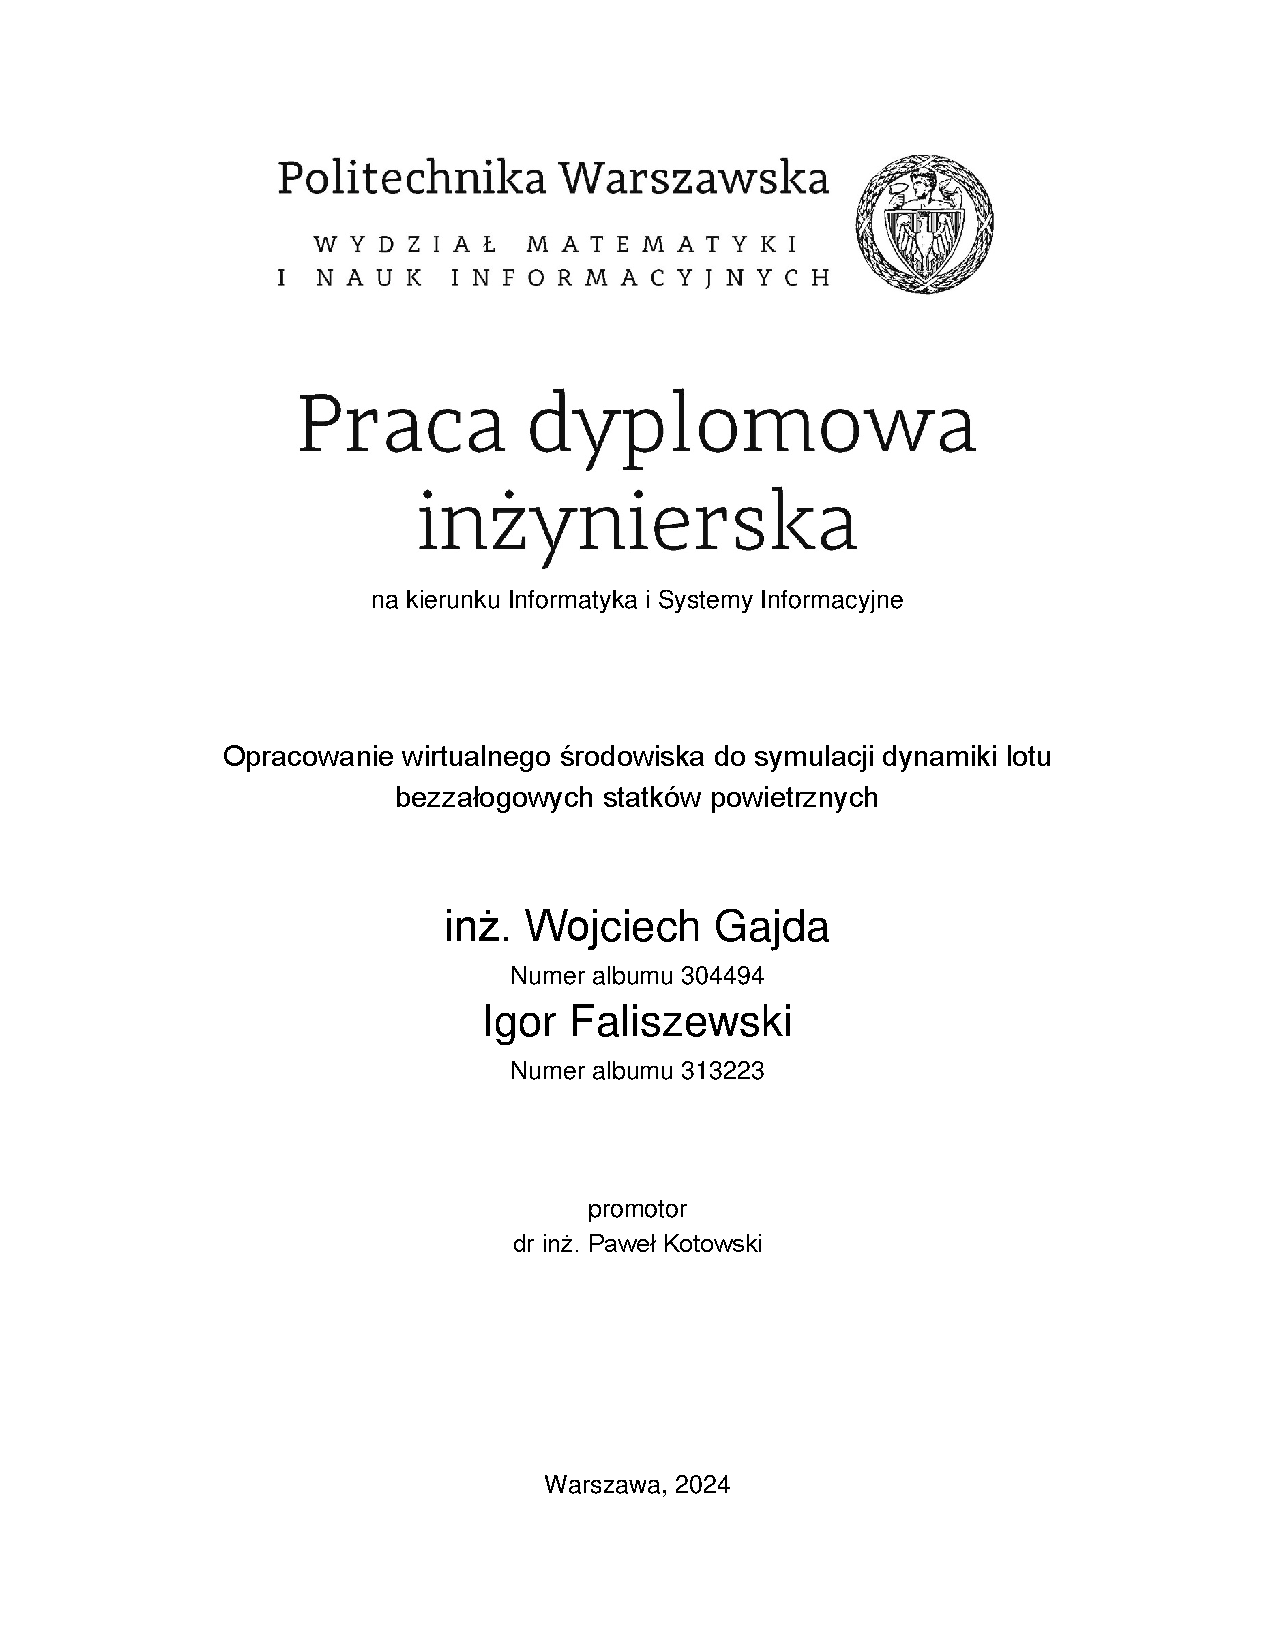
\includepdf[pages=-]{first_page.pdf}

\section*{Streszczenie}
Niniejsza specyfikacja stanowi opis systemu przeznaczonego do symulacji dynamiki lotu bezzałogowych statków powietrznych. System pozwala na prowadzenie symulacji lotu w czasie rzeczywistym, który dodatkowo jest prezentowany jest w postaci trójwymiarowej wizualizacji. W trakcie wykonywania lotu logowane są dane i mogą zostać wykorzystane do analizy lotu. Opracowany został uniwersalny model dynamiki pozwalający na swobodną konfigurację parametrów statku. Obejmuje on modyfikację właściwości mechanicznych, aerodynamicznych oraz konfigurację zespołów napędowych i~wpływu czynników zewnętrznych. Symulacja dynamiki rozszerzona została o system sterowania. System został zaprojektowany w sposobu ułatwiający zmianę parametrów statków i symulacji, tworzenie nowych konfiguracji statków oraz tworzenie i strojenie systemów sterowania. Przykładowych modelami, które mogą zostać zasymulowane są: stałopłatowiec, wielowirnikowiec i rakiety. 

\section*{Słowa kluczowe}

symulacja, grafika komputerowa 3D, bezzałogowy statek powietrzny, model dynamiki ruchu

\newpage

\section*{Abstract}

\section*{Keywords}

\newpage
\tableofcontents

\section{Historia zmian}

\renewcommand{\arraystretch}{1.5}
\begin{table}[!h]
\centering
\begin{tabular}{|m{0.12\textwidth}|m{0.12\textwidth}|m{0.20\textwidth}|m{0.45\textwidth}|} 
\hline
\rowcolor{Gray}
Nr rewizji & Data & Autor & Opis \\
 \hline
  0.0 & 10.08.23 & Wojciech Gajda & Utworzenie dokumentu, podstawowa struktura \\ 
\hline
  0.1 & 11.10.23 & Wojciech Gajda & Dostosowanie dokumentu do wymogów edytorskich, dodanie streszczenia \\ 
\hline
  0.2 & 15.10.23 & Wojciech Gajda \newline Igor Faliszewski & Dodanie  słownika, specyfikacji, analizy SWOT i bibliografii \\ 
\hline
  1.0 & 16.10.23 & Wojciech Gajda \newline Igor Faliszewski & Wydanie zgłoszone do L1 \\
\hline
  1.1 & 16.10.23 & Wojciech Gajda \newline Igor Faliszewski & Wprowadzenie poprawek po L1 \\
\hline
  1.2 & 5.11.23 & Wojciech Gajda \newline Igor Faliszewski & Wydanie zgłoszone do L2 \\
\hline
  1.3 & 5.12.23 & Wojciech Gajda \newline Igor Faliszewski & Wydanie zgłoszone do L3/L4 \\
\hline
  1.4 & 10.12.23 & Wojciech Gajda \newline Igor Faliszewski & Wydanie zgłoszone do L5 \\
\hline
  2.0 & 30.12.23 & Wojciech Gajda \newline Igor Faliszewski & Dostosowanie dokumentu do formatu pracy inżynierskiej \\
\hline
\end{tabular}
\caption{Historia zmian}
\label{changelog}
\end{table}

\section{Słownik pojęć}

\textbf{Statek powietrzny} -- urządzenie zdolne do unoszenia się (lotu) w atmosferze. Statek powietrzny jest zdolny w sposób aktywny wpływać na kierunek i prędkość lotu. W przeciwieństwie do formalnej definicji termin obejmuje również konstrukcję niewykorzystujące oddziaływania powietrza w locie (rakiety).\\

\textbf{Bezzałogowy statek powietrzny, BSP} -- statek powietrzny, który nie wymaga do lotu załogi obecnej na pokładzie oraz nie ma możliwości zabierania pasażerów, pilotowany zdalnie lub wykonujący lot autonomicznie.\\ 

\textbf{Pocisk} -- obiekt wystrzelony lub upuszczony ze statku powietrznego, nieposiadający własnego napędu. Porusza się na wskutek oddziaływania pola grawitacji i wpływu powietrza. Nie posiada wyróżnionej orientacji.\\

\textbf{Ładunek} -- pocisk, na ogół upuszczany, który pozostaje związany z statkiem powietrznym na sprężysto-tłumiącej linie. \\

\textbf{Stan obiektu} -- Opis położenia, orientacji i prędkości obiektu (pocisku lub statku powietrznego). Stan może zostać rozszerzony o dodatkowe informacje, takie jak: prędkości obrotowe poszczególnych silników, położenie powierzchni sterowych itd. \\

\textbf{Silnik fizyczny, silnik dynamiki} -- program komputerowy, którego zadaniem jest obliczenie położenia, orientacji i prędkości (kinematyki) statków powietrznych w zależności od sił działających na obiekt (dynamiki). \\

\textbf{Regulator} -- układ odpowiedzialny za generowanie rozkazów sterujących w oparciu o aktualny i zadany stan obiektu.\\

\textbf{Silnik graficzny} -- program komputerowy, którego zadaniem jest wizualizacja stanu obiektów i otoczenia.\\

\textbf{Agregator} --  program komputerowy, którego zadaniem jest zarządzaniem stanem aplikacji, obsługa przyłączających się aplikacji klienckich i zarządzanie procesami.\\

\textbf{Zasoby wizualizacji, assety} -- Modele i grafiki niezbędne do pracy aplikacji klienckiej.

\chapter{Wstęp}

\section{O projekcie}

Symulacje komputerowe dynamiki ruchu stanowią użyteczne narzędzie w pracach inżynierskich. Pozwalają na analizę poprawności działania układu mechanicznego przed jego wyprodukowaniem. W szczególności w zagadnieniu jakim jest projektowanie bezzałogowych statków powietrznych, zastosowanie symulacji pozwala zminimalizować koszty wytworzenia poprawnie działającego systemu.

\section{Przegląd istniejących rozwiązań}

Historia symulatorów lotu sięga lat 30. XX wieku. Pierwotnie zastosowanie symulatorów sprowadzało się do szkolenia pilotów cywilnych i wojskowych. W znanej obecnie formie kompletne symulatory lotu stanowią rozbudowane systemy integrujące wysokiej klasy oprogramowanie z peryferiami mającymi wierne odwzorowanie kokpitu kierowanej maszyny. Symulatory wykorzystywane do treningu pilotów podlegają rygorystycznym regulacjom prawnym i na ogół ich zadaniem jest odwzorowanie jednej konkretnej maszyny. Równolegle uproszczone wersje symulatorów zaczęły zyskiwać popularność w zastosowaniu cywilnym, jako element rozrywki. W szczególności gry komputerowe związane z lotem bardzo często poświęcały zgodność z rzeczywistością na rzecz lepszych odczuć użytkownika.\\

Na rynku dostępnych jest wiele środowisk symulacyjnych o różnym stopniu szczegółowości. Pełne systemy lotu stanowią produkt komercyjny projektowany na indywidualne zamówienie. Do najpopularniejszych dostępnych systemów sprzedawanych jako zamknięte oprogramowanie należą m. in.:

\begin{itemize}
\item Microsoft Flight Simulator -  seria komputerowych symulatorów lotu pozwalająca na symulację pilotowania różnych statków powietrznych. Założeniem jest wierne odtworzenie zachowania statków powietrznych, warunków pogodowych, jak również samych maszyn,
\item VBS (Arma) - środowisko symulacyjne do wizualizacji pola walki,
\item Warthunder - darmowa gra komputerowa wprowadzająca znaczną ilość historycznych i współczesnych modeli samolotów, których parametry zostały oparte na dostępnych i odtajnionych danych,
\item RealFlight - modelarski symulator lotu.
\end{itemize}

Istnieją również rozwiązania typu open-source, realizujące jedynie poszczególne zadania:

\begin{itemize}
\item JSBsim - rozbudowany silnik dynamiki lotu działający w czasie rzeczywistym,
\item Ardupilot, INAV, Betaflight - kompletne systemy sterowania dla modeli zdalnie sterowanych.
\end{itemize}

\section{Cel projektu}

Celem niniejszej projektu jest opracowanie wirtualnego środowiska do symulacji dynamiki lotu bezzałogowych statków powietrznych. System implementuje rozbudowany model dynamiki statków powietrznych wyposażonych w silniki rotorowe, silniki odrzutowe, powierzchnie nośne i powierzchnie sterowe. Pozwala na przeprowadzenie lotu symulowanym obiektem, którego parametry określane są przez konfigurację podaną przez użytkownika. Oprócz lotu system udostępnia dodatkowe funkcjonalności, takie jak możliwość strzału, upuszczenia ładunku, lotu z ładunkiem, rozpoznawania kolizji z otoczeniem.\\

Oprogramowanie ma stanowić zaawansowane narzędzie inżynierskie. Docelowym odbiorcą mają być zespoły R\&D opracowujące nowe konstrukcje latające lub prowadzące prace nad nowatorskimi systemami sterowania. System umożliwia zamodelowanie rzeczywistego modelu latającego i symulację jego lotu przed rzeczywistymi lotami próbnymi, co w rezultacie pozwoli na zminimalizowanie kosztów prototypowania. System rejestruje wiele parametrów lotu, umożliwiając późniejszą analizę. Potencjalnymi odbiorcami systemu są uczelnie i instytuty naukowe, a także przedsiębiorstwa prowadzące prace badawczo-rozwojowe. Ze względu na różnorodność zagadnień badanych przez wspomniane zespoły, trudno przygotować oprogramowanie uniwersalne. Z tego powodu system zostanie udostępniony na otwartej licencji MIT, aby umożliwić zespołom dostosowanie go do własnych potrzeb. Dla ułatwienia dalszego rozwoju projektu duży nacisk położony zostanie na przejrzystą implementację i realizację wzorców możliwych do ponownego użycia.\\

Otwarta licencja umożliwia również wykorzystanie systemu do celów rekreacyjnych i hobbistycznych. Szczególnym przypadkiem są modelarze, posiadający nierzadko znaczną wiedzę domenową i budujący swoje modele ze znaczną dbałością o szczegóły. Projektowany system może stanowić dla nich zamiennik profesjonalnego oprogramowania, które ze względu na koszty licencji pozostawało dla nich niedostępne. Specyfika oprogramowania pozwala na użytkowanie go również w roli gry komputerowej. Oprócz wartości rozrywkowej korzystanie z symulatora pozwala rozwijać umiejętności pilotażu, co przenosi się na rzeczywiste modele. Planowane jest wprowadzenie kilku funkcjonalności, których rolą jest jedynie polepszenie odczuć użytkownika aplikacji i zwiększenie przyjemności z korzystania z systemu.\\

\newpage
\section{Wymagania funkcjonalne}

Wyróżniono trzech aktorów korzystających z systemu: Użytkownika, Analityka i Developera. Użytkownik to osoba o najmniejszej wiedzy domenowej. Korzysta z systemu odpowiednio skonfigurowanego i przygotowanego. Rolą Użytkownika jest wykonywanie lotów i realizacja określonej misji. Można porównać go do gracza. Użytkownik korzysta z systemu, aby nauczyć się pilotować określony BSP lub aby trenować zaawansowane manewry, np. atak na poruszający się cel lub precyzyjne upuszczenie ładunku. Analityk to osoba posiadająca rozbudowaną wiedzę teoretyczną z zakresu lotnictwa. Odpowiedzialny jest za identyfikacje i wprowadzenie parametrów modelu BSP i przygotowanie konfiguracji do lotu. Po odbytym locie może zwalidować poszczególne aspekty lotu poprzez analizę zarejestrowanych logów. Developer to osoba posiadająca podstawową wiedzę domenową i rozumie kod źródłowy systemu. Rolą developera jest dostosowanie systemu na potrzeby swojego przedsiębiorstwa. Zakłada się, że główną modyfikacją jest implementacja własnych algorytmów sterowania. Developer ma dostęp do całego kodu źródłowego, przez co jego możliwości są nieograniczone.\\

\textbf{Użytkownik:}
\begin{itemize}[noitemsep,nolistsep]
	\item może uruchomić symulację lotu,
	\item może wybrać jedną z dostępnych konfiguracji BSP,
	\item może dołączyć do symulacji wraz z innymi użytkownikami,
	\item może dodać konfigurację własnego kontrolera
	\item może w trakcie lotu wystrzelić pocisk,
	\item może w trakcie lotu upuścić ładunek i przenosić go na elastycznej linie,
	\item może zderzyć się z ścinami mapy, innym BSP lub pociskiem,
	\item może połączyć się zdalnie z wykorzystaniem protokołu TCP/IP,
	\item może odczytać stan swojego BSP z GUI,
	\item może zmienić widok z kamery,
	\item może uruchomić radio w grze.
\end{itemize}

\textbf{Analityk:}
\begin{itemize}[noitemsep,nolistsep]
	\item może przygotować nową konfigurację drona,
	\item może analizować logi z wykonanych lotów,
	\item może zaplanować otoczenie symulacji, wybrać mapę i ustalić warunki atmosferyczne,
	\item może wygenerować nową mapą w oparciu o dane geograficzne.
\end{itemize}

\textbf{Developer:}
\begin{itemize}[noitemsep,nolistsep]
	\item może dodać i zarządzać istniejącymi algorytmami sterowania,
	\item implementować nowe funkcjonalności systemu.
\end{itemize}

\newpage
\section{Wymaganie niefunkcjonalne}

W tabeli (\ref{non_func}) przedstawiono wymagania niefunkcjonalne, które musi spełniać oprogramowanie.

\renewcommand{\arraystretch}{1.2}
\begin{table}[!h]
	\centering
	\begin{tabular}{|m{0.03\textwidth}|m{0.18\textwidth}|m{0.02\textwidth}|m{0.65\textwidth}|} 
		\hline
		\rowcolor{Gray}		\multicolumn{2}{|c|}{Wymagania} & No. & Opis \\
		\hline
		\centering \multirow{9}{*}{\rotatebox[origin=c]{90}{Usability}}
		&\multirow{1}{*}{Używalność} 
		& 1 & Użytkownik jest w stanie dopasować rozmiar okna wizualizacji i interfejsu do swoich potrzeb i ograniczeń sprzętu. \\
		\cline{3-4}
		& & 2 & Serwer da się uruchomić natywnie na Unixie lub w wirtualnym kontenerze Docker, a wizualizacja działa na wirtualnej maszynie Javy. \\
		\cline{3-4}
		& & 3 & Komunikacja między serwerem, a wizualizacją powinna pozwalać na responsywne sterowanie BSP. \\
		\cline{2-4}
		& \multirow{1}{*}{Ergonomia} 
		& 4 & Interfejs użytkownika powinien być przejrzysty i korzystać ze standardowych liczników wykorzystywanych w~lotnictwie.  \\
		\cline{3-4}
		& & 5 & Konfiguracja kontrolera powinna odbyć się bez znajomości użytkownika z interpretacją wejścia przez system.  \\
		\hline
		\centering \multirow{3.5}{*}{\rotatebox[origin=c]{90}{Reliability}}
		& \multirow{1}{*}{Dokładność} 
		& 6 & Dokładność symulacji powinna zależeć wyłącznie od błędów obliczeń i dokładności wprowadzonych parametrów. \\
		\cline{2-4}
		& \multirow{1}{*}{Sprawdzalność} 
		& 7 & Zgodność symulacji z rzeczywistością da się sprawdzić poprzez analizę logów oraz przez subiektywną opinię analityka. \\
		\hline
		\centering \multirow{1}{*}{\rotatebox[origin=c]{90}{Perf.}}
		& \multirow{1}{*}{Przepustowość} 
		& 8 & Wydajność serwera powinna skalować się względem liczby aktualnie symulowanych BSP. \\
		\hline
		\centering \multirow{7}{*}{\rotatebox[origin=c]{90}{Supportability}}
		& \multirow{1}{*}{Konserwacja} 
		& 9 &Systemy sterowania, elementy interfejsu i moduły konfigurowalne powinny być tak zaprojektowanie aby dodawanie nowych oraz modyfikacja istniejących była prosta i szybka.  \\
		\cline{3-4}
		& & 10 & System powinien być podzielony na moduły, które można niezależnie modyfikować. \\
		\cline{2-4}
		& \multirow{1}{*}{Audytowalność} 
		& 11 & W czasie lotu serwer powinien zapisywać logi z symulacji. \\
		\cline{2-4}
		& \multirow{1}{*}{Instalowalność} 
		& 12 & Proces instalacji serwera powinien być dobrze opisany i~prosty. Niewymagany w przypadku wizualizacji. \\
		\cline{2-4}
		& \multirow{1}{*}{Konfigurowalność} 
		& 13 & Oprogramowanie powinno umożliwiać konfigurację serwera, wizualizacji, modeli, kontrolerów, parametrów BSP. \\
		\hline
	\end{tabular}
	\caption{Wymaganie niefunkcjonalne - FURPS}
	\label{non_func}
\end{table}

\newpage
\section{Ocena ryzyka -- analiza SWOT}

\begin{table}[!h]
	\begin{tikzpicture}
		\renewcommand{\arraystretch}{1.2}
		\setlist{left=1em,parsep=0.5ex,after=\smallskip}
		\def\myw{7.5cm}
		\matrix[SWOT] 
		{
			\& |[fill=black!10]|\renewcommand{\arraystretch}{1.3}\begin{tabular}{Wc{\myw}Wc{\myw}}
				Pozytywne & Negatywne\\ 
			\end{tabular}\\
			Wewnętrzne
			\& \begin{tabular}{p{\myw}p{\myw}}
				\textbf{Silne strony:} \begin{itemize}
					\item przejrzysta implementacja zgodna z paradygmatami programowania obiektowego,
					\item modułowość projektu, pozwalająca na modyfikację poszczególnych komponentów bez konieczności przebudowy całego projektu,
					\item uniwersalny model dynamiki statków powietrznych, pozwalający na obliczenia w czasie rzeczywistym.
				\end{itemize}
				& 
				\textbf{Słabe strony:} \begin{itemize}
					\item ograniczony czas projektu może skutkować niedopracowaniami we wdrożonych funkcjonalnościach,
					\item obliczenia symulacji i kolizji obywają się na CPU, co może ograniczać wydajność,
					\item model matematyczny jest mniej dokładny niż rozbudowana symulacja mechaniki płynów.
			\end{itemize} \end{tabular}\\
			Zewnętrzne \& \begin{tabular}{p{\myw}p{\myw}}
				\textbf{Szanse:} \begin{itemize}
					\item dzięki udostępnieniu systemu na otwartej licencji, możliwe jest wykorzystanie wypracowanych rozwiązań w przyszłych projektach,
					\item system może stanowić narzędzie ułatwiające opracowanie i testowanie nowatorskich systemów sterowania,
					\item system może stanowić bezpłatną alternatywę dla komercyjnych symulatorów lotu.
				\end{itemize} & \textbf{Zagrożenia:} \begin{itemize}
					\item język Rust wykorzystany w UAV\_aggregator może przestać być wspierany na przestrzeni najbliższych lat,
					\item trudności z identyfikacja wiarygodnych współczynników modelu dynamiki,
					\item rozbudowany system może okazać się trudny w obsłudze dla użytkownika.
					
			\end{itemize} \end{tabular}\\
		};
	\end{tikzpicture}
	\caption{Analiza SWOT}
	\label{swot}
\end{table}



\include{chapters/theory\_1}

\include{chapters/theory\_2}

\section{Specyfikacja}


\subsection{Cel projektu}

Celem niniejszej projektu jest opracowanie wirtualnego środowiska do symulacji dynamiki lotu bezzałogowych statków powietrznych. System implementuje rozbudowany model dynamiki statków powietrznych wyposażonych w silniki rotorowe, silniki odrzutowe, powierzchnie nośne i powierzchnie sterowe. Pozwala na przeprowadzenie lotu symulowanym obiektem, którego parametry określane są przez konfigurację podaną przez użytkownika. Oprócz lotu system udostępnia dodatkowe funkcjonalności, takie jak możliwość strzału, upuszczenia ładunku, lotu z ładunkiem, rozpoznawania kolizji z otoczeniem.\\

Oprogramowanie ma stanowić zaawansowane narzędzie inżynierskie. Docelowym odbiorcą mają być zespoły R\&D opracowujące nowe konstrukcje latające lub prowadzące prace nad nowatorskimi systemami sterowania. System umożliwia zamodelowanie rzeczywistego modelu latającego i symulację jego lotu przed rzeczywistymi lotami próbnymi, co w rezultacie pozwoli na zminimalizowanie kosztów prototypowania. System rejestruje wiele parametrów lotu, umożliwiając późniejszą analizę. Potencjalnymi odbiorcami systemu są uczelnie i instytuty naukowe, a także przedsiębiorstwa prowadzące prace badawczo-rozwojowe. Ze względu na różnorodność zagadnień badanych przez wspomniane zespoły, trudno przygotować oprogramowanie uniwersalne. Z tego powodu system zostanie udostępniony na otwartej licencji MIT, aby umożliwić zespołom dostosowanie go do własnych potrzeb. Dla ułatwienia dalszego rozwoju projektu duży nacisk położony zostanie na przejrzystą implementację i realizację wzorców możliwych do ponownego użycia.\\

Otwarta licencja umożliwia również wykorzystanie systemu do celów rekreacyjnych i hobbistycznych. Szczególnym przypadkiem są modelarze, posiadający nierzadko znaczną wiedzę domenową i budujący swoje modele ze znaczną dbałością o szczegóły. Projektowany system może stanowić dla nich zamiennik profesjonalnego oprogramowania, które ze względu na koszty licencji pozostawało dla nich niedostępne. Specyfika oprogramowania pozwala na użytkowanie go również w roli gry komputerowej. Oprócz wartości rozrywkowej korzystanie z symulatora pozwala rozwijać umiejętności pilotażu, co przenosi się na rzeczywiste modele. Planowane jest wprowadzenie kilku funkcjonalności, których rolą jest jedynie polepszenie odczuć użytkownika aplikacji i zwiększenie przyjemności z korzystania z systemu.\\

\newpage
\subsection{Wymagania funkcjonalne}

Wyróżniono trzech aktorów korzystających z systemu: Użytkownika, Analityka i Developera. Użytkownik to osoba o najmniejszej wiedzy domenowej. Korzysta z systemu odpowiednio skonfigurowanego i przygotowanego. Rolą Użytkownika jest wykonywanie lotów i realizacja określonej misji. Można porównać go do gracza. Użytkownik korzysta z systemu, aby nauczyć się pilotować określony BSP lub aby trenować zaawansowane manewry, np. atak na poruszający się cel lub precyzyjne upuszczenie ładunku. Analityk to osoba posiadająca rozbudowaną wiedzę teoretyczną z zakresu lotnictwa. Odpowiedzialny jest za identyfikacje i wprowadzenie parametrów modelu BSP i przygotowanie konfiguracji do lotu. Po odbytym locie może zwalidować poszczególne aspekty lotu poprzez analizę zarejestrowanych logów. Developer to osoba posiadająca podstawową wiedzę domenową i rozumie kod źródłowy systemu. Rolą developera jest dostosowanie systemu na potrzeby swojego przedsiębiorstwa. Zakłada się, że główną modyfikacją jest implementacja własnych algorytmów sterowania. Developer ma dostęp do całego kodu źródłowego, przez co jego możliwości są nieograniczone.\\

\textbf{Użytkownik:}
\begin{itemize}[noitemsep,nolistsep]
	\item może uruchomić symulację lotu,
	\item może wybrać jedną z dostępnych konfiguracji BSP,
	\item może dołączyć do symulacji wraz z innymi użytkownikami,
	\item może dodać konfigurację własnego kontrolera
	\item może w trakcie lotu wystrzelić pocisk,
	\item może w trakcie lotu upuścić ładunek i przenosić go na elastycznej linie,
	\item może zderzyć się z ścinami mapy, innym BSP lub pociskiem,
	\item może połączyć się zdalnie z wykorzystaniem protokołu TCP/IP,
	\item może odczytać stan swojego BSP z GUI,
	\item może zmienić widok z kamery,
	\item może uruchomić radio w grze.
\end{itemize}
\ \\

\textbf{Analityk:}
\begin{itemize}[noitemsep,nolistsep]
	\item może przygotować nową konfigurację drona,
	\item może analizować logi z wykonanych lotów,
	\item może zaplanować otoczenie symulacji, wybrać mapę i ustalić warunki atmosferyczne,
	\item może wygenerować nową mapą w oparciu o dane geograficzne.
\end{itemize}
\ \\

\textbf{Developer:}
\begin{itemize}[noitemsep,nolistsep]
	\item może dodać i zarządzać istniejącymi algorytmami sterowania,
	\item implementować nowe funkcjonalności systemu.
\end{itemize}
\ \\


\newpage
\subsection{Wymaganie niefunkcjonalne}

W tabeli (\ref{non_func}) przedstawiono wymagania niefunkcjonalne, które musi spełniać oprogramowanie.

\renewcommand{\arraystretch}{1.5}
\begin{table}[!h]
	\centering
	\begin{tabular}{|m{0.03\textwidth}|m{0.21\textwidth}|m{0.025\textwidth}|m{0.68\textwidth}|} 
		\hline
		\rowcolor{Gray}		\multicolumn{2}{|c|}{Wymagania} & No. & Opis \\
		\hline
		\centering \multirow{9}{*}{\rotatebox[origin=c]{90}{Usability}}
		&\multirow{1}{*}{Używalność} 
		& 1 & Użytkownik jest w stanie dopasować rozmiar okna wizualizacji i interfejsu do swoich potrzeb i ograniczeń sprzętu. \\
		\cline{3-4}
		& & 2 & Serwer da się uruchomić natywnie na Unixie lub w wirtualnym kontenerze Docker, a wizualizacja działa na wirtualnej maszynie Javy. \\
		\cline{3-4}
		& & 3 & Komunikacja między serwerem, a wizualizacją powinna pozwalać na responsywne sterowanie BSP. \\
		\cline{2-4}
		& \multirow{1}{*}{Ergonomia} 
		& 4 & Interfejs użytkownika powinien być przejrzysty i korzystać ze standardowych liczników wykorzystywanych w~lotnictwie.  \\
		\cline{3-4}
		& & 5 & Konfiguracja kontrolera powinna odbyć się bez znajomości użytkownika z interpretacją wejścia przez system.  \\
		\hline
		\centering \multirow{3.5}{*}{\rotatebox[origin=c]{90}{Reliability}}
		& \multirow{1}{*}{Dokładność} 
		& 6 & Dokładność symulacji powinna zależeć wyłącznie od błędów obliczeń i dokładności wprowadzonych parametrów. \\
		\cline{2-4}
		& \multirow{1}{*}{Sprawdzalność} 
		& 7 & Zgodność symulacji z rzeczywistością da się sprawdzić poprzez analizę logów oraz przez subiektywną opinię analityka. \\
		\hline
		\centering \multirow{1}{*}{\rotatebox[origin=c]{90}{Perf.}}
		& \multirow{1}{*}{Przepustowość} 
		& 8 & Wydajność serwera powinna skalować się względem liczby aktualnie symulowanych BSP. \\
		\hline
		\centering \multirow{7}{*}{\rotatebox[origin=c]{90}{Supportability}}
		& \multirow{1}{*}{Konserwacja} 
		& 9 &Systemy sterowania, elementy interfejsu i moduły konfigurowalne powinny być tak zaprojektowanie aby dodawanie nowych oraz modyfikacja istniejących była prosta i szybka.  \\
		\cline{3-4}
		& & 10 & System powinien być podzielony na moduły, które można niezależnie modyfikować. \\
		\cline{2-4}
		& \multirow{1}{*}{Audytowalność} 
		& 11 & W czasie lotu serwer powinien zapisywać logi z symulacji. \\
		\cline{2-4}
		& \multirow{1}{*}{Instalowalność} 
		& 12 & Proces instalacji serwera powinien być dobrze opisany i~prosty. Niewymagany w przypadku wizualizacji. \\
		\cline{2-4}
		& \multirow{1}{*}{Konfigurowalność} 
		& 13 & Oprogramowanie powinno umożliwiać konfigurację serwera, wizualizacji, modeli, kontrolerów, parametrów BSP. \\
		\hline
	\end{tabular}
	\caption{Wymaganie niefunkcjonalne - FURPS}
	\label{non_func}
\end{table}

\subsection{Architektura}

System został podzielony na moduły. Poszczególne moduły odpowiadają obiektom z domeny projektu i realizują następujące zadania:\\

\textbf{UAV\_physic\_engine} -- moduł odpowiedzialny symulację dynamiki statku powietrznego, uwzględniając wszystkie jego właściwości mechaniczne i wpływ otoczenia. Oblicza stan pojedynczego BSP w czasie rzeczywistym. \\

\textbf{UAV\_controller} -- moduł reprezentujący system sterowania statkiem powietrznym. Interpretuje stan statków powietrznych i buduje symulacje otoczenie. Symuluje działanie czujników pomiarowych, systemu filtracji, algorytmów nawigacji pokładowej oraz systemów sterowania i stabilizacji. Bezpośrednio wpływa na zachowanie symulacji dynamiki.\\

\textbf{UAV\_drop\_physic} -- moduł odpowiedzialny za obliczenie dynamiki pocisków. Oblicza stan wszystkich pocisków aktywnych w symulacji.\\

\textbf{UAV\_aggregator} -- moduł agregujący moduły symulacyjne z wizualizacją. Zarządza pracą pozostałych modeli i wprowadza niektóre zagadnienia otoczenia takie jak atmosferę, połączenia miedzy BSP, a ładunkami oraz kolizje.\\

\textbf{UAV\_server} -- definicja wirtualnego kontenera, odpowiedzialna zabudowanie wszystkich modułów składających się na serwer, tj. wszystkie z wyłączeniem wizualizacji. Ze zbudowanych modułów budowany jest obraz kontenera. Umożliwia to uruchomienie serwera na dowolnej maszynie wspierającej daną konteneryzację.\\

\textbf{UAV\_visualization} -- moduł odpowiedzialny za wyświetlenie  interfejsu użytkownika oraz obecnego stanu symulacji. Przekazuje dane wejściowe z kontrolera do systemu. Stanowi interfejs komunikacji użytkownika z systemem. \\

\textbf{UAV\_map\_generator} -- skrypt automatyzujący proces generowania mapy, w oparciu o dane geograficzne. \\

\newpage

\subsection{Opis działania systemu}

W centralnym punkcie aplikacji znajduje się moduł agregatora. Stanowi on główną część serwera, jest aplikacją konsolową i nie posiada interfejsu graficznego. Jest zawsze uruchamiany jako pierwszy. Po rozpoczęciu pracy agregatora uruchamiany jest moduł "drop physic" jako podproces, a agregator nawiązuje z nim połączenie. Oba moduły pozostają w stanie bezczynności do momentu podłączenia się pierwszego użytkownika. Nowy użytkownik dodawany jest przez uruchomienie wizualizacji. Po uruchomieniu wizualizacji, komunikuje się ona z serwerem i prosi o~utworzenie nowego statku powietrznego. W odpowiedzi na to żądanie, agregator uruchamia jako swoje podprocesy "physic engine" i "controller".Następnie para procesów synchronizuje się ze sobą i rozpoczyna symulację. Każdemu symulowanemu statkowi powietrznemu odpowiada para procesów "physic engine" i "controller". Ponadto każdy statek jest kontrolowany z poziomu konkretnej wizualizacji.\\

W trakcie pracy systemu agregator pełni rolę pośrednika w komunikacji między wizualizacją a procesami silnika fizycznego i regulatora. Przesyła instrukcje sterujące z wizualizacji do odpowiedniej symulacji fizycznej, agreguje stany ze wszystkich aktywnych symulacji i przesyła je z powrotem do wizualizacji. Ponadto zarządza procesami strzału, upuszczania ładunku i kolizji.\\

Po odłączeniu się wizualizacji od serwera, procesy związane z danym statkiem są zamykane.


\subsection{Opis komponentów}

Kod poszczególnych modułów systemu został w całości opisany z wykorzystaniem narzędzi do dokumentowania kodu: Doxygen, JavaDoc i Rust Doc. Dla poszczególnych modułów wygenerowane zostały opisy klas oraz funkcji i załączone do pracy jako dokumenty PDF lub strony HTML.

\newpage

\subsection{Komunikacja}

Moduły komunikują się między sobą poprzez kolejki ZeroMQ\cite{zmqguide}. ZeroMQ to uniwersalna implementacja różnych wzorów komunikacji niezależna od języka i warstwy transportowej. Istnieją oficjalne biblioteki ZeroMQ przeznaczone do wykorzystania w projektach w językach  C++, Rust, Java, Python i wielu innych. Jako warstwa transportowa wykorzystane mogą być mechanizmy komunikacji wewnątrzprocesowej, międzyprocesowej i protokół TCP/IP oraz dowolne ich kombinację. Wzorami dostępnymi w kolejkach ZeroMQ, które zostaną wykorzystane w projekcie są:

\begin{itemize}
\item PUB--SUB -- jednokierunkowa komunikacja publikujący --  subskrybujący. Jest to połączenie jeden do wielu.  Wielu subskrybujących ma możliwość podłączenia się do jednego publikującego i zasubskrybowania określonych wiadomości (zdefiniowanych przez prefix). Publikujący rozsyła wiadomości do wszystkich podłączonych subskrybentów, którzy subskrybują dany typ wiadomości.

\item PAIR--PAIR -- uniwersalne połączenie jeden do jeden. Tworzy połączenie dwóch socketów, umożliwiające dwukierunkową komunikacje. Stanowi bezpośredni odpowiednich Unixowych pipe'ów lub surowego protokołu TCP.

\item REQ--REP -- model komunikacji klient serwer w której serwer (REP -- replyer) odpowiada na zapytania klienta (REQ -- requester). W modelu wielu klientów może odpytywać serwer, a ich żądania są kolejno obsługiwane i wysyłana jest na nie odpowiedź.
\end{itemize}

Oprócz wyżej przedstawionych istnieje również wiele wariacji modeli komunikacji pozwalające m. in. na rozdzielanie pracy na wiele serwerów (load balance) lub przekierowywanie wiadomości ze zmianą warstwy transportowej lub podsłuchem (proxy).\\

Rysunek (\ref{comm}) prezentuje poszczególne moduły oraz kanały komunikacji. Na niebiesko zaznaczone zostały kolejki TCP/IP, a na czerwono kolejki wykorzystujące mechanizmy IPC. Dla zwiększenia czytelności, kolejki w warstwie miedzy procesowej nie zostały zaznaczone na rysunku.

\newpage
 \begin{figure}[!h]
  \centering
  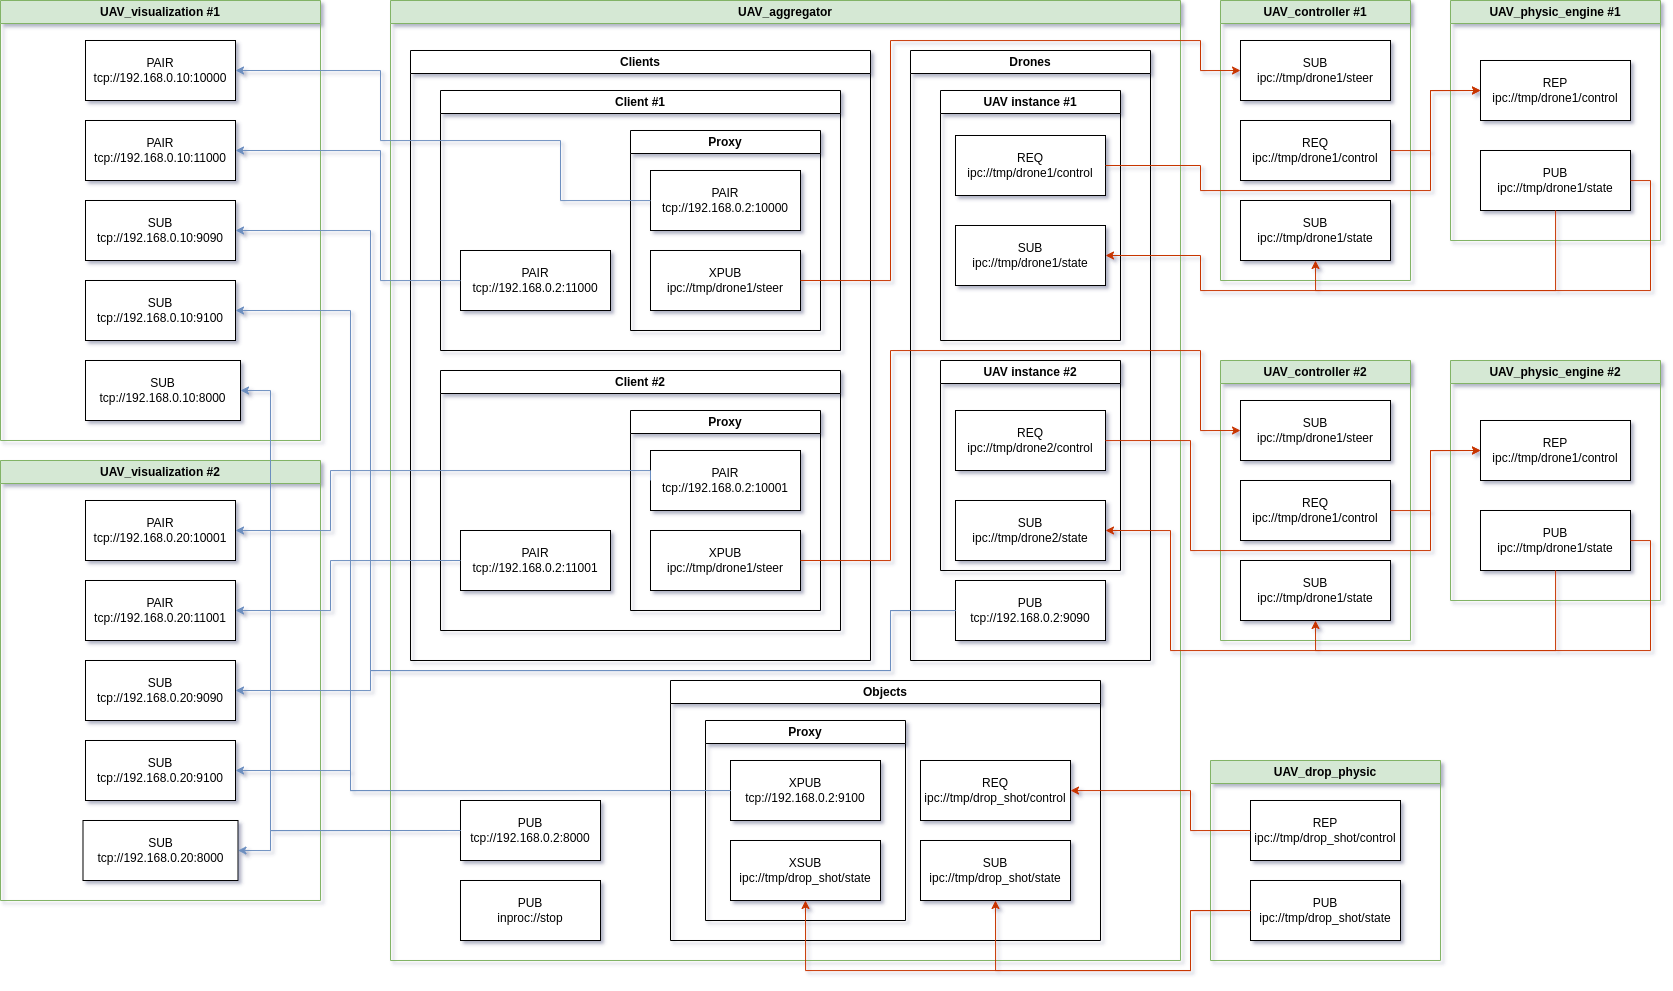
\includegraphics[width=1.2\textwidth, angle=90]{ZMQinMINIUAV.drawio.png}
  \caption{Schemat komunikacji}
  \label{comm}
 \end{figure}

\newpage

\subsection{Graficzny interfejs użytkownika}

Graficzny interfejs użytkownika składa się z interfejsu serwera oraz interfejsu wizualizacji. 

\subsubsection*{Serwer}

Interfejs serwera zawiera komunikaty dotyczące pracy agregatora oraz otrzymywane od poszczególnych modułów, które są wyświetlane w oknie konsoli. Komunikaty są dodatkowo oznaczone różniącymi się kolorami dla poszczególnych modułów, jak pokazano na rysunkach (\ref{gui_server1}), (\ref{gui_server2}) i (\ref{gui_server3}).

\subsubsection*{Wizualizacja}

Interfejs graficzny wizualizacji składa się z okna konfiguracji przypisań kontrolera pokazanego na rysunku (\ref{gui_bindings1}), ekranu ładowania widocznego na rysunku (\ref{gui_loading}) oraz właściwego widoku wizualizacji ukazanego na rysunkach (\ref{gui_game1}), (\ref{gui_game2}), (\ref{gui_game3}) i (\ref{gui_game4}). \\

Graficzny interfejs użytkownika w wizualizacji składa się z widoku jednej z kamer do wyboru oraz kokpitu. Kokpit w lewym dolnym rogu zawiera radar pozwalający na wykrycie BSP w okolicy. W prawym dolnym rogu znajduje się schemat silników BSP, gdzie możemy odczytać ich prędkości obrotowe. W prawym górnym rogu jest pokazany stan wyposażenia kontrolowanego BSP. Ponadto na kokpicie na dole ekranu znajduje się sztuczny horyzont, którego wizualizacja zgodna jest z powszechnie stosowaną konstrukcją. Pozwala on na uzyskanie informacji o pozycji BSP w przestrzeni, jego orientacji i prędkościach. W lewym górnym rogu sztucznego horyzontu znajduje się obecny tryb lotu BSP. Użytkownik może również włączyć tryb mapy, aby zobaczyć swoje położenia w świecie symulacji.

\newpage
\begin{figure}[!h]
	\centering
	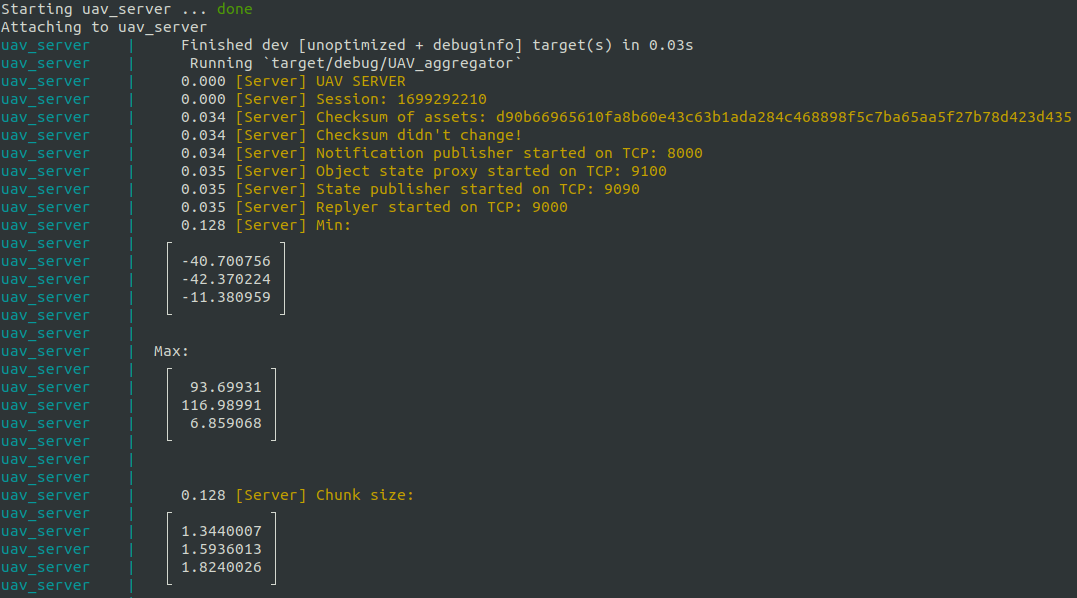
\includegraphics[width=1\textwidth]{gui_server_start.png}
	\caption{Interfejs graficzny serwera w momencie startu.}
	\label{gui_server1}
\end{figure}

\begin{figure}[!h]
	\centering
	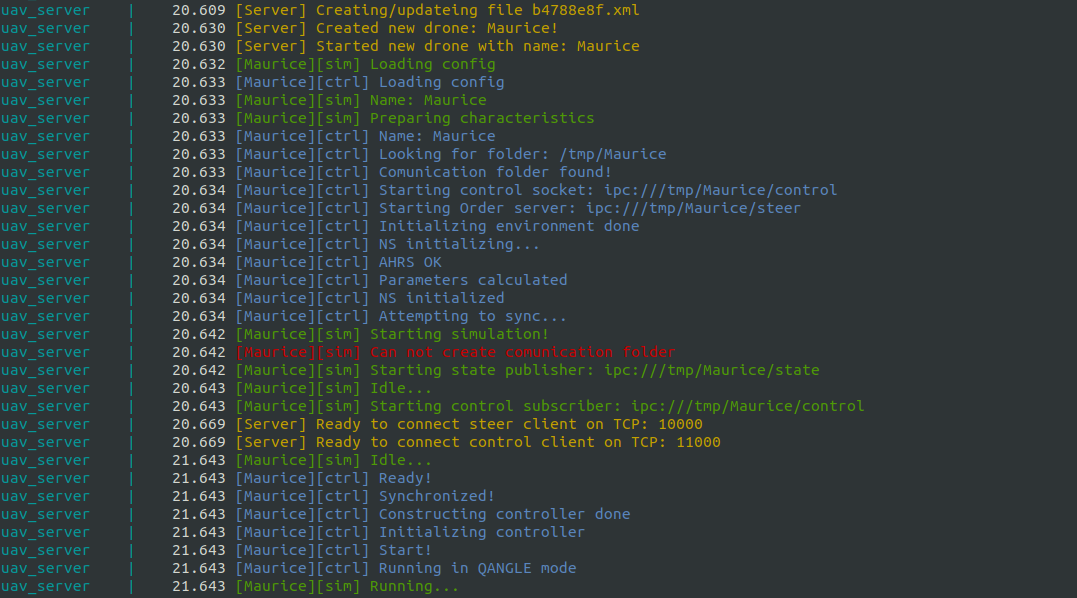
\includegraphics[width=1\textwidth]{gui_server_drone.png}
	\caption{Interfejs graficzny serwera w momencie dołączenia nowego klienta wizualizacji.}
	\label{gui_server2}
\end{figure}

\begin{figure}[!h]
	\centering
	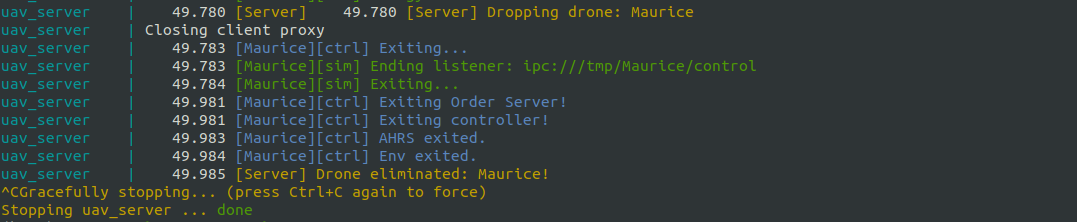
\includegraphics[width=1\textwidth]{gui_server_exit.png}
	\caption{Interfejs graficzny serwera w momencie wyłączenia serwera.}
	\label{gui_server3}
\end{figure}
\begin{figure}[!h]
	\centering
	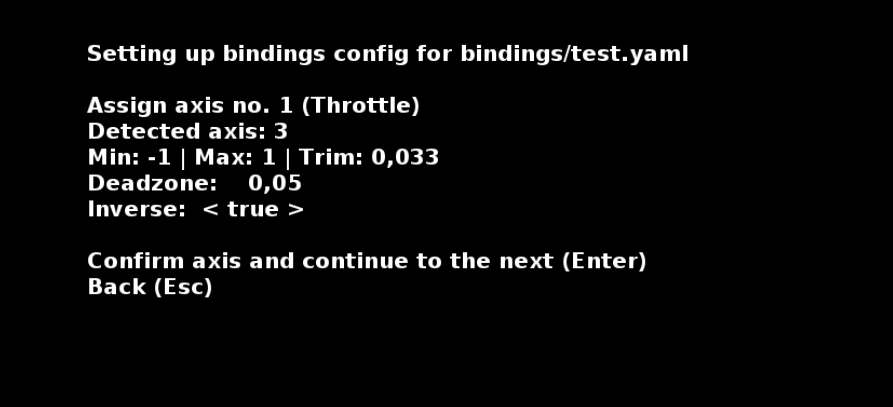
\includegraphics[width=1\textwidth]{bindings1.png}
	\caption{Ekran przypisania osi sterowania.}
	\label{gui_bindings1}
\end{figure}

\begin{figure}[!h]
	\centering
	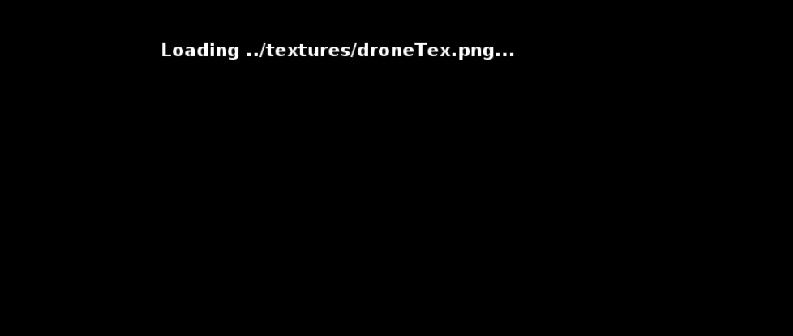
\includegraphics[width=1\textwidth]{loading_screen.png}
	\caption{Ekran ładowania.}
	\label{gui_loading}
\end{figure}

\newpage
\begin{figure}[!h]
	\centering
	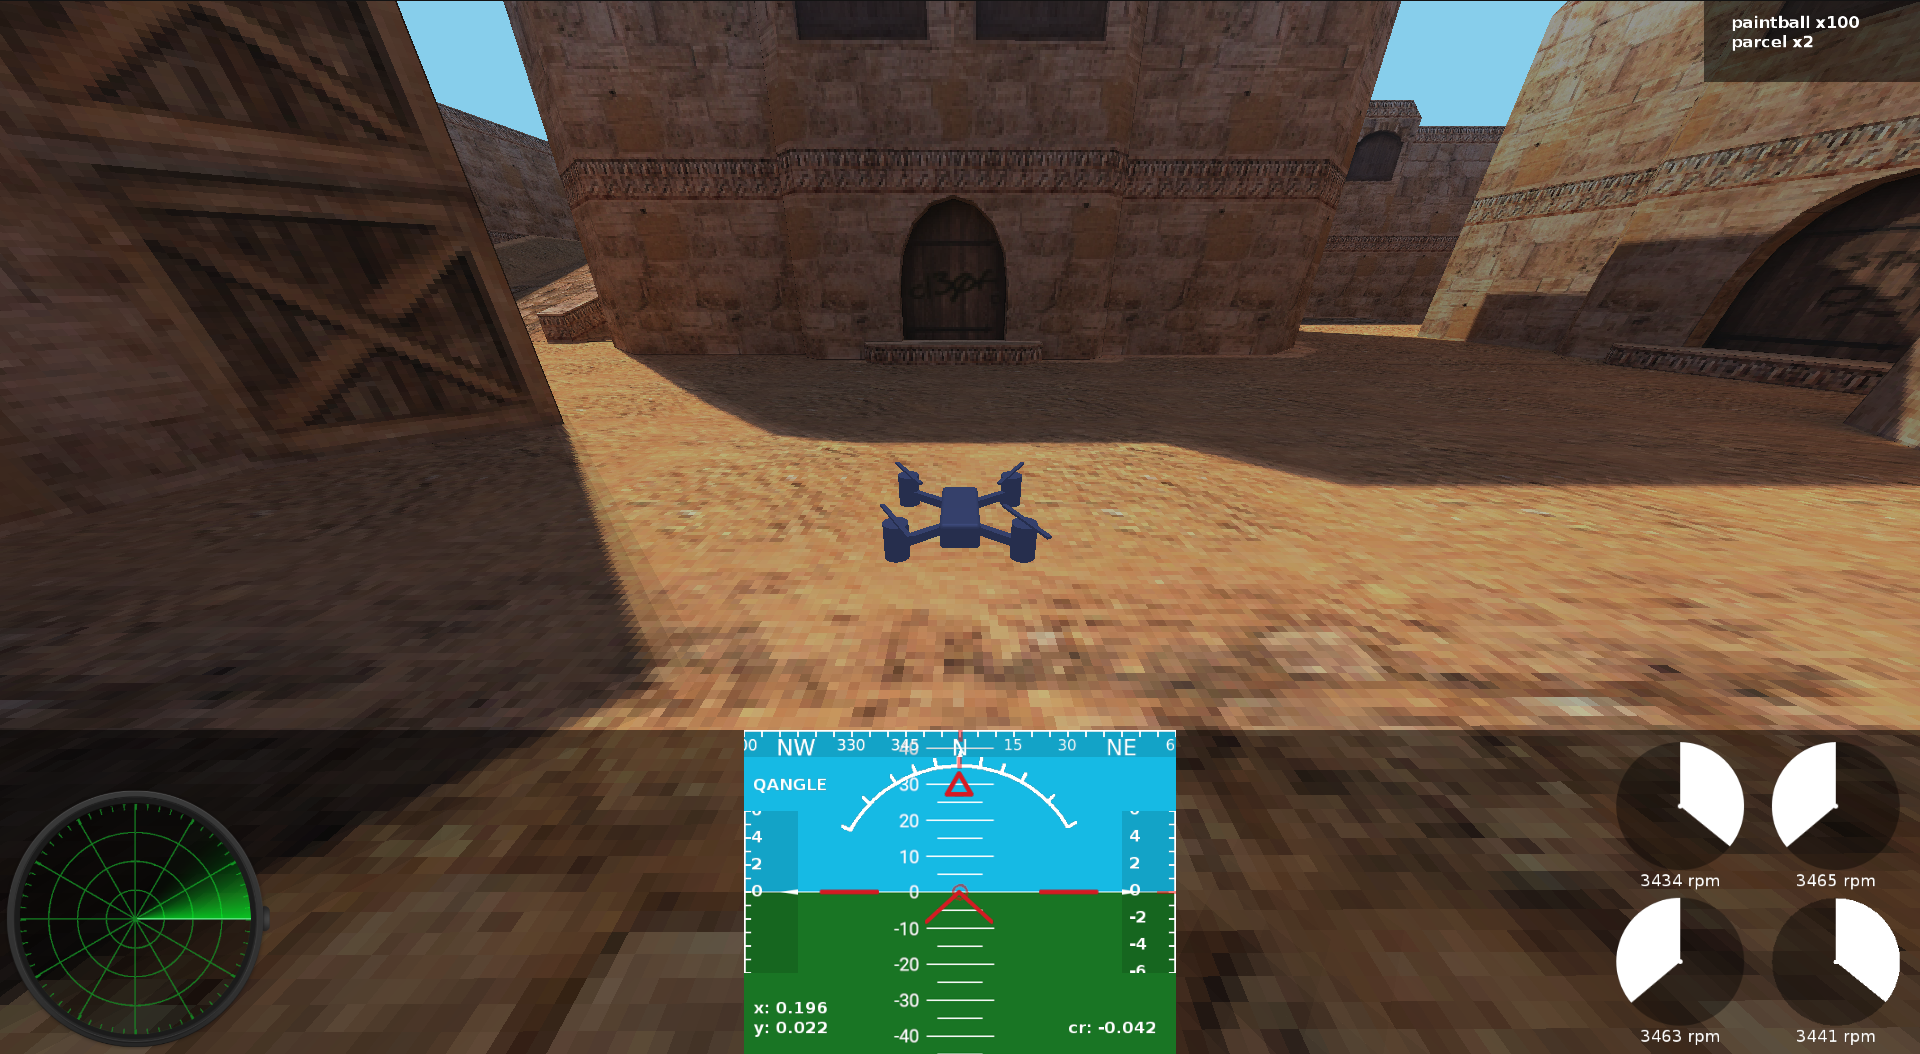
\includegraphics[width=1\textwidth]{game_view.png}
	\caption{Interfejs graficzny wizualizacji w widoku trzecioosobowym.}
	\label{gui_game1}
\end{figure}

\begin{figure}[!h]
	\centering
	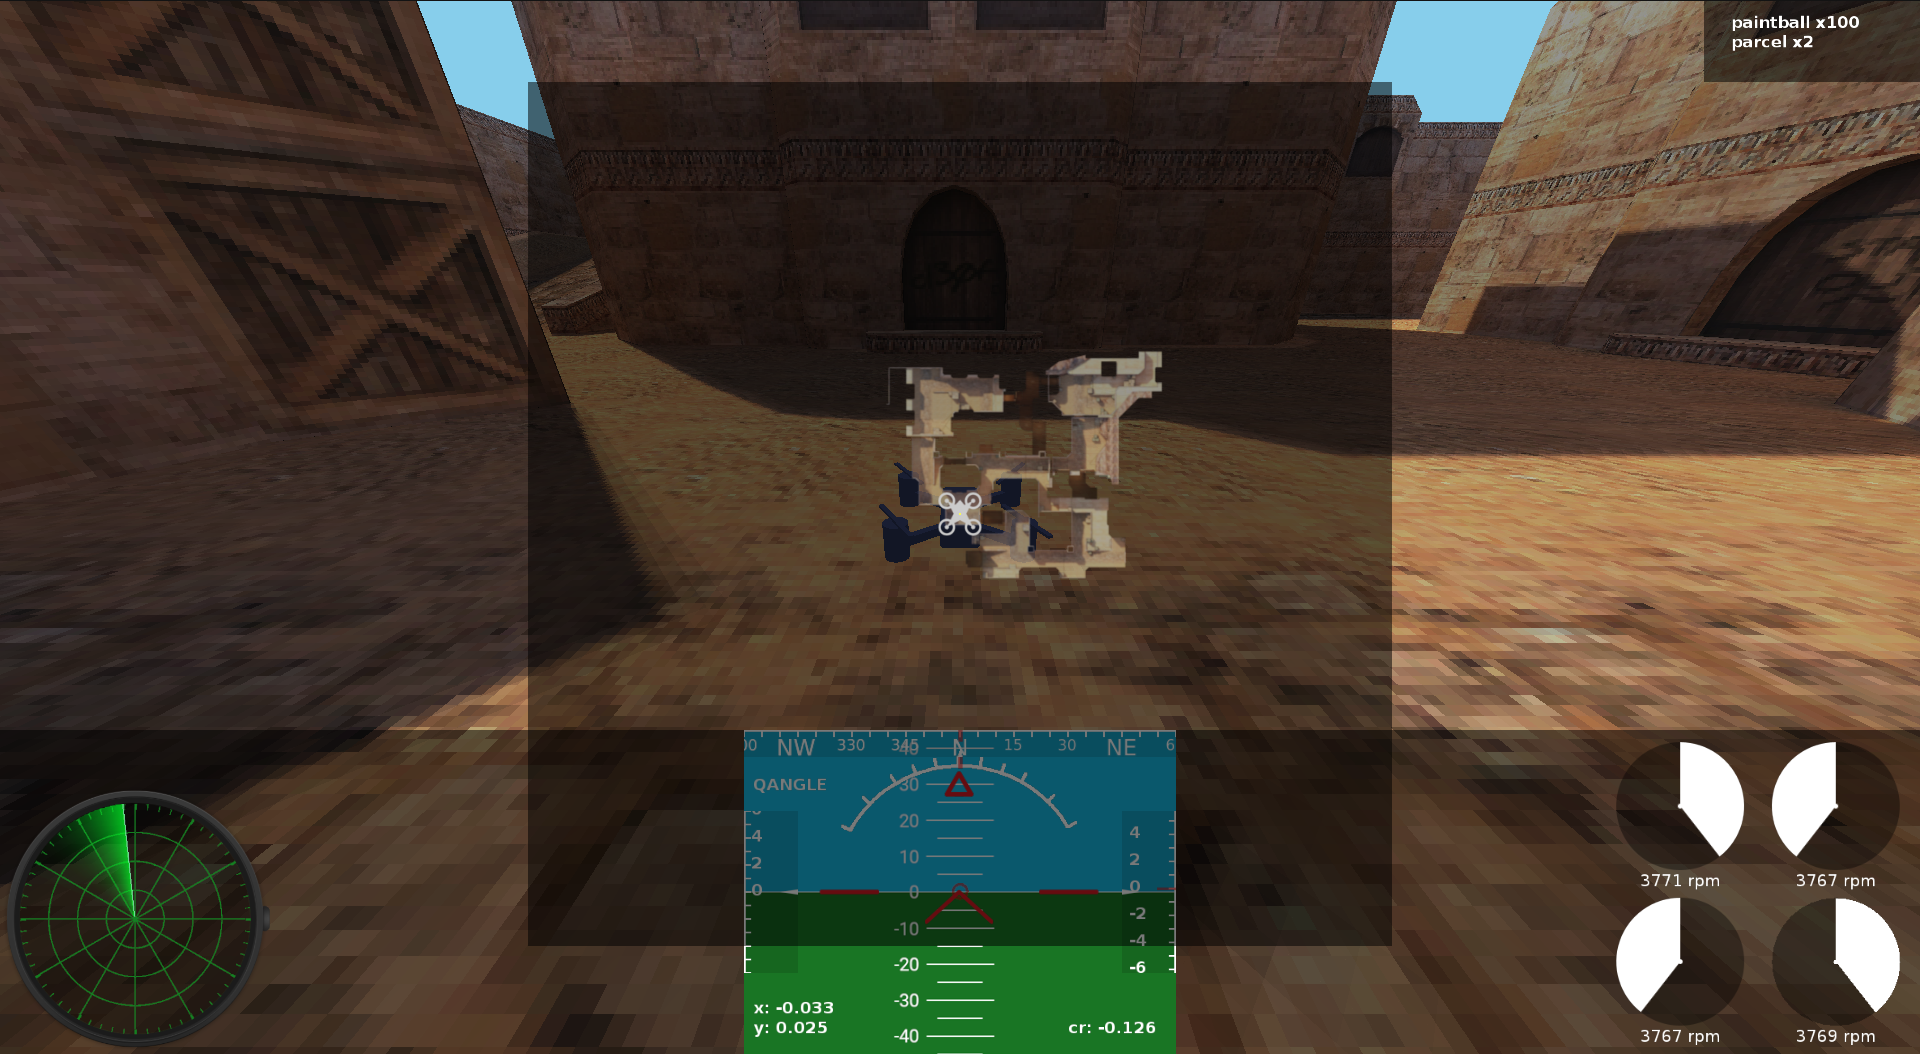
\includegraphics[width=1\textwidth]{game_view_map.png}
	\caption{Interfejs graficzny wizualizacji z włączonym widokiem mapy.}
	\label{gui_game2}
\end{figure}

\newpage
\begin{figure}[!h]
	\centering
	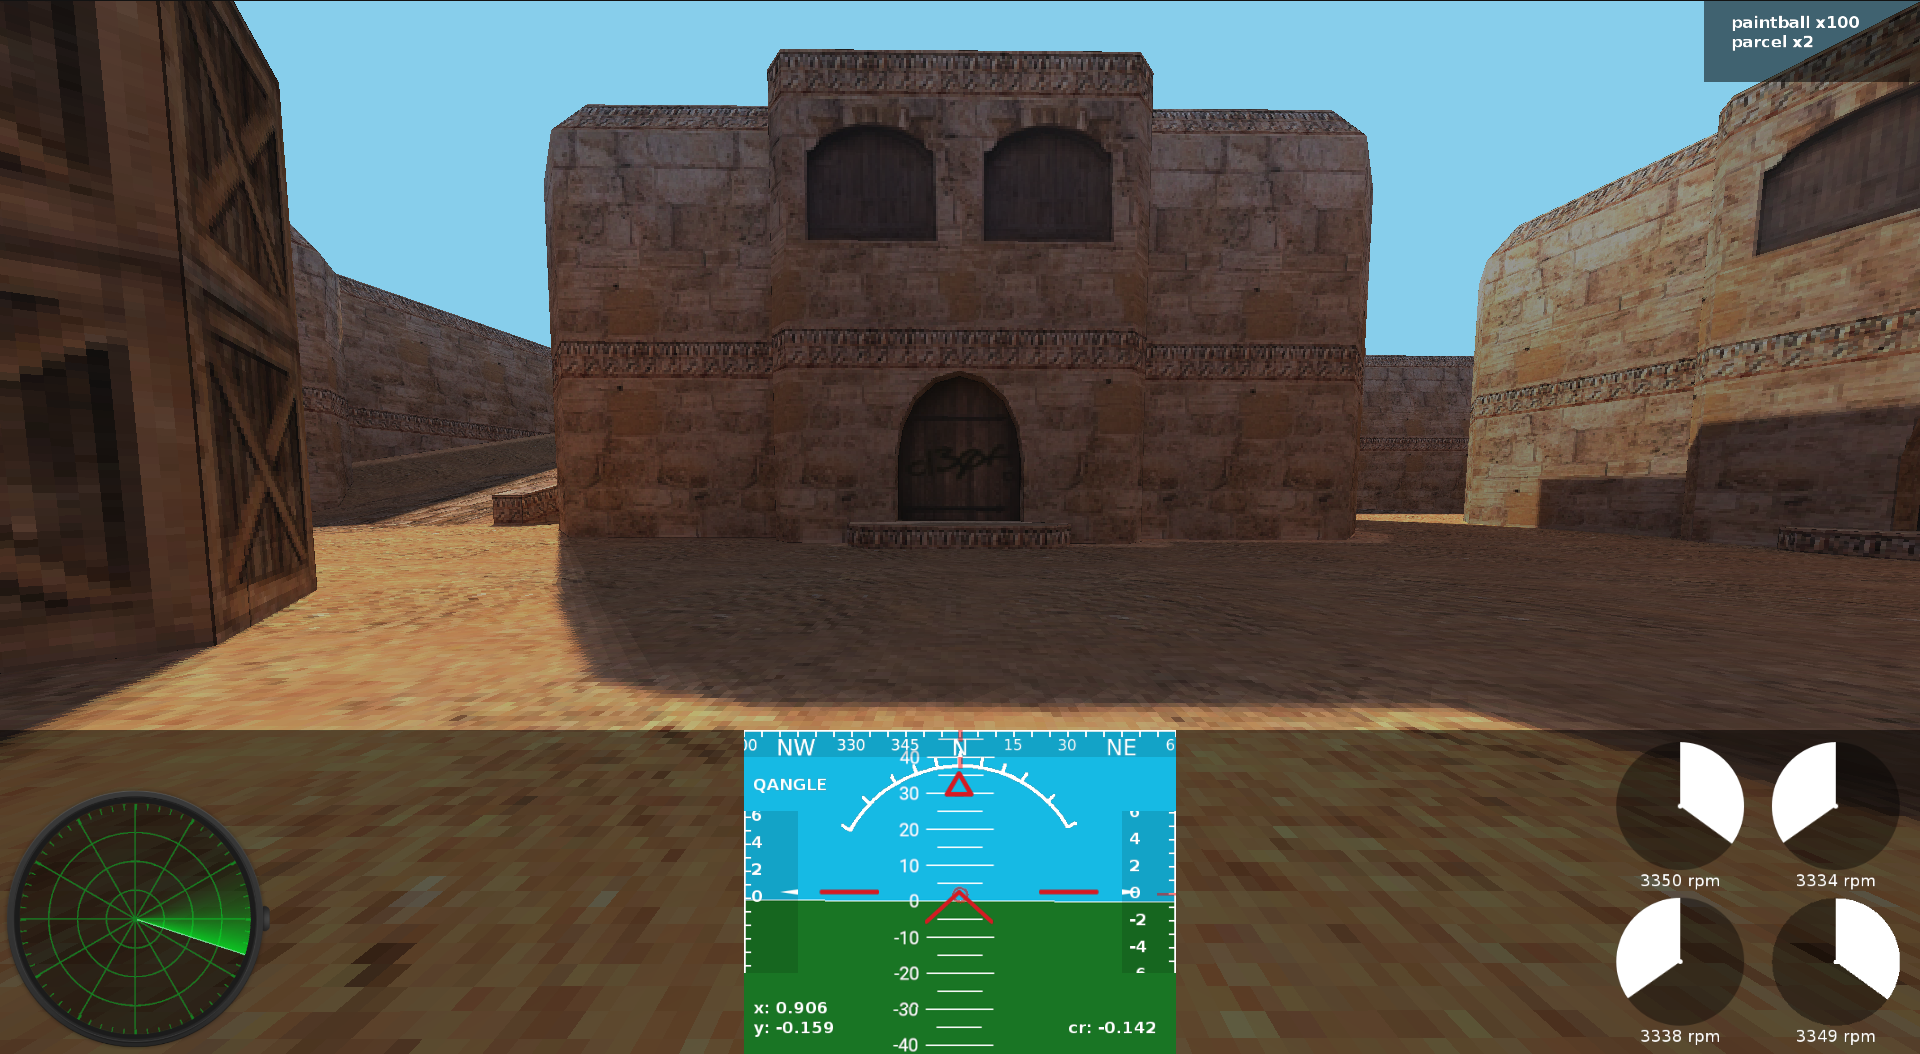
\includegraphics[width=1\textwidth]{game_view_fpp.png}
	\caption{Interfejs graficzny wizualizacji w widoku pierwszoosobowym.}
	\label{gui_game3}
\end{figure}

\begin{figure}[!h]
	\centering
	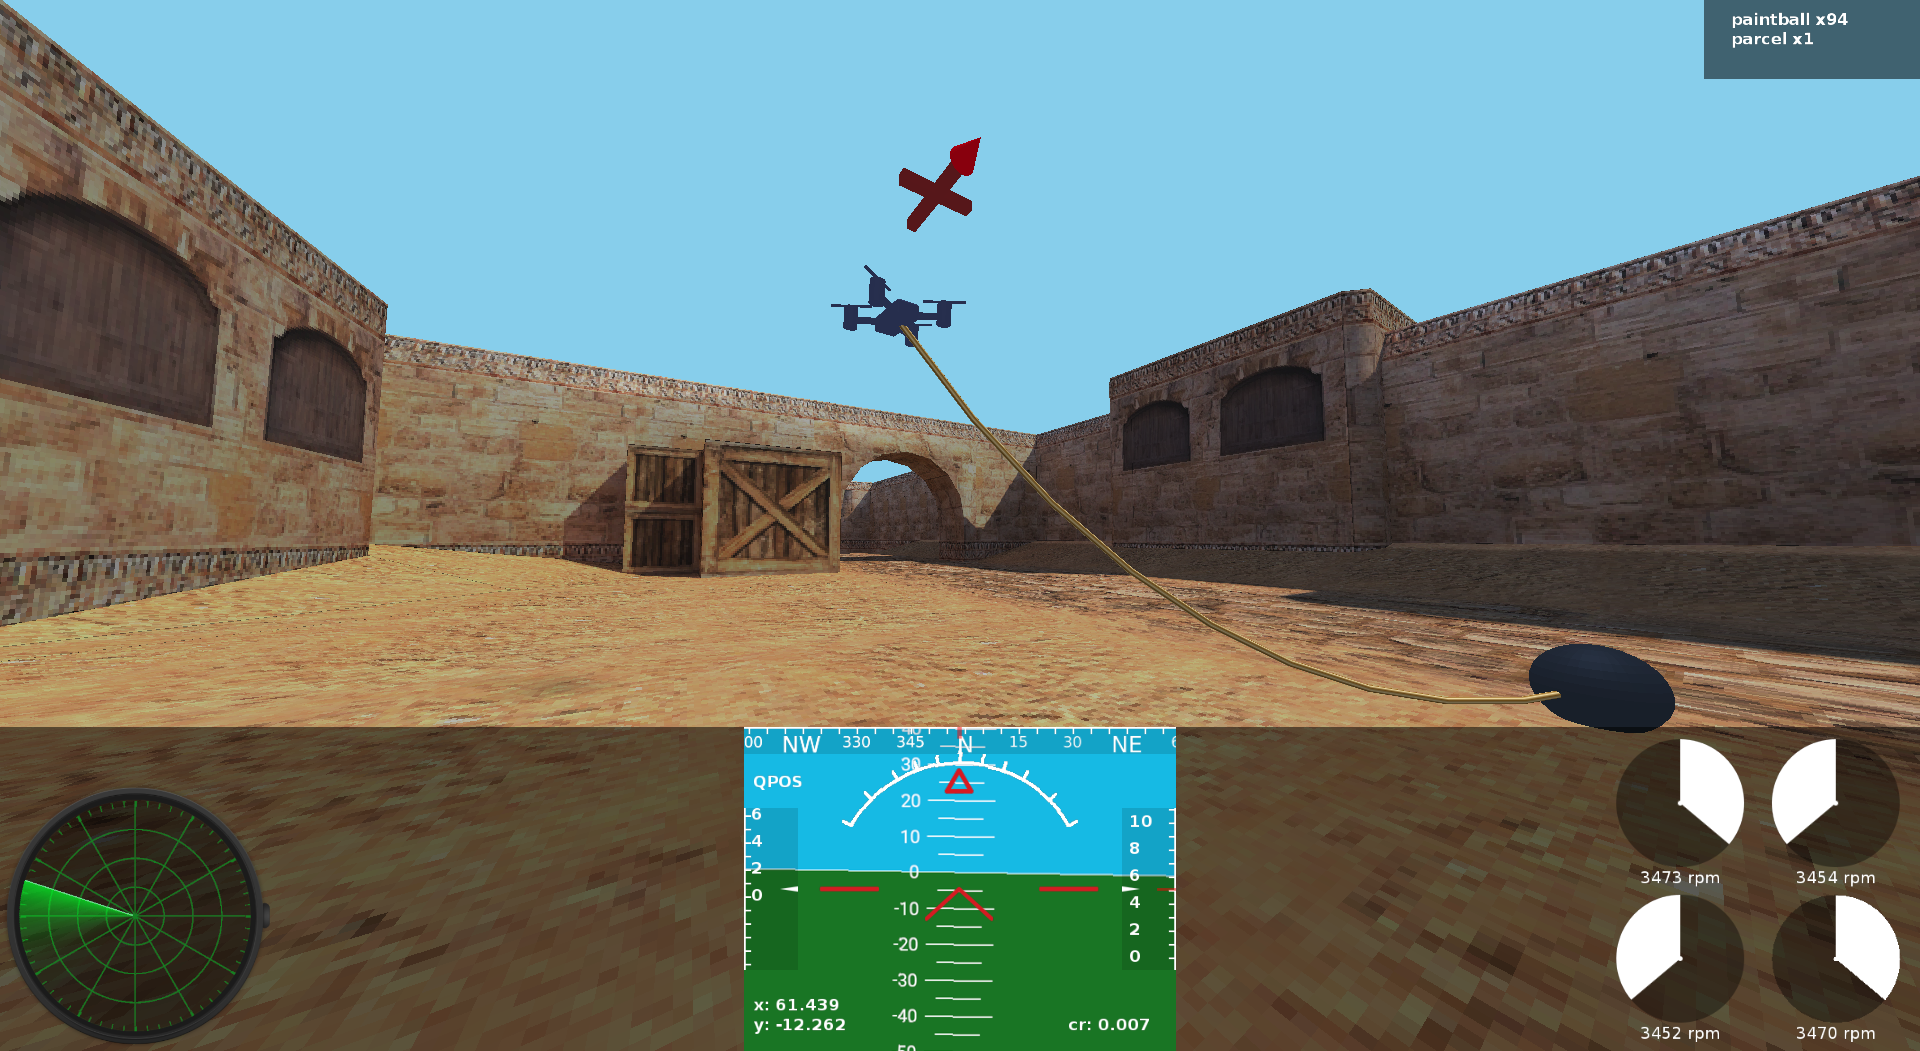
\includegraphics[width=1\textwidth]{game_view_rope.png}
	\caption{Interfejs graficzny wizualizacji w widoku obserwatora i pozycyjnym trybie lotu z opuszczonym ładunkiem na linie.}
	\label{gui_game4}
\end{figure}

\newpage
\subsection{Interfejs zewnętrzny}

Konfiguracja systemu przed uruchomieniem odbywa się poprzez modyfikację plików konfiguracyjnych i zasobów (asset'ów). Pliki konfiguracyjne dotyczą:

\begin{itemize}
\item Parametrów symulowanego statku powietrznego --\\ UAV\_aggregator/configs/template.xml
\item Parametrów agregatora -- UAV\_aggregator/configs/config.yaml
\item Parametrów wizualizacji -- UAV\_visualization/config.yaml
\item Parametrów kontrolera --  UAV\_visualization/bindings/template.yaml
\item Opisu dostępnych trybów lotu --\\ UAV\_aggregator/assets/data/available\_control\_modes.yaml
\end{itemize}

Pliki konfiguracyjne zostały w całości skomentowane przy pomocy komentarzy odpowiednich dla plików XML oraz YAML  i załączone do pracy.\\


Zasoby zawierają modele i grafiki niezbędne do pracy wizualizacji. Wersja zasobów to pierwsze 8 znaków sumy kontrolnej, która jest generowana na podstawie zawartości assetów i przekazywana wizualizacji przez serwer. Pozwala to użytkownikowi pobrać brakujące zasoby w razie, gdy ich jeszcze nie posiada. Pobrana zawartość jest umieszczana w katalogu od nazwie będącej wersją zasobu. Zasób zawiera następujące katalogi:

\begin{itemize}

\item \textbf{Drones} -- folder zawierający modele 3D statków powietrznych. Zawiera foldery odpowiadające poszczególnym BSP. Nazwa folderu jest tożsama z nazwą BSP.
\begin{itemize}
\item \textbf{\textbf{\textit{NazwaModeluBSP}}} -- Katalog zawierający modele wraz z teksturami dla konkretnego modelu BSP w folderach \textbf{model} i \textbf{textures}.
\end{itemize}

\item \textbf{Maps} -- folder zawierający modele 3D map, które mogą zostać wykorzystane w symulacji. Zawiera foldery odpowiadające poszczególnym mapą. Nazwa folderu jest tożsama z nazwą mapy.
\begin{itemize}
	\item \textbf{\textbf{\textit{NazwaMapy}}} -- Katalog modeli danej mapy. Zawiera modele oraz tekstury mapy w folderach \textbf{model} i \textbf{textures}. W folderze \textbf{model} dodatkowo znajduje się obraz mapy z lotu ptaka pod nazwą "minimap.png".
\end{itemize}

\item \textbf{Data} -- folder zawierający wspólne pliki konfiguracyjne. Obecnie zawiera następujące pliki:
\begin{itemize}
	\item "available\_control\_modes.yaml" -- Plik konfiguracyjny zawierający dozwolone tryby kontroli lotu.
\end{itemize}

\item \textbf{Core} -- folder zawierający pozostałe modele 3D i elementy interfejsu. Zawiera następujące podfoldery:
\begin{itemize}
	\item \textbf{GUI} -- Grafiki niezbędne do wyświetlenia elementów interfejsu graficznego użytkownika.
	\item \textbf{projectile} -- Model i tekstury pocisku w katalogach \textbf{model} i \textbf{textures}.
	\item \textbf{xMark} -- Model i tekstury markera 3D w katalogach \textbf{model} i \textbf{textures}.
\end{itemize}

\end{itemize}

W katalogach \textbf{model} zawarty jest model obiektu w postaci pliku z rozszerzeniem GLTF, a więc "model.gltf" wraz z odpowiadającym mu "model.bin" oraz pliku z rozszerzeniem OBJ: "model.obj". Plik GLTF wykorzystywany jest w wizualizacji, a OBJ służy rozpoznawaniu kolizji.\\


W zasobie znajduje się również tekstura domyślna ładowana w przypadku nieznalezienia wymaganej tekstury.\\


\newpage


\subsection{Dobór technologii} \label{technologies}

Do realizacji poszczególnych modułów wybrane zostały następujące narzędzia programistyczne i biblioteki zewnętrzne.\\


\textbf{UAV\_physic\_engine, UAV\_controller i UAV\_drop\_physic}\\

Ze względu na duży nakład obliczeniowy -- symulacja w czasie rzeczywistym z krokiem całkowania rzędu 1ms -- wybrany został język C++. Z uwagi na swoją wydajność i elastyczność stanowi on naturalny wybór w wydajnych symulacjach komputerowych. Dodatkowo wykorzystane zostały następujące biblioteki:
\begin{itemize}[noitemsep,nolistsep]
	\item Eigen -- biblioteka zawierająca elementy algebry liniowej: macierze, wektory i~związane z nimi algorytmy. Eigen stawia na wydajność poprzez wykorzystanie rozkładów typu SIMD, przy 		jednoczesnym zachowaniu przejrzystej składni,
	\item ZeroMQ -- binding biblioteki libzmq dla języka C++. Libzmq jest bazową biblioteką implementującą kolejki ZeroMQ w języku C,
	\item RapidXML -- biblioteka do parsowania plików XML,
	\item Cxxopts -- biblioteka do interpretowania argumentów wejściowych programu.
\end{itemize}
\  \\
\textbf{UAV\_aggregator}\\

Do realizacji modułu agregatora wykorzystany zostanie język Rust. Pozwala on na tworzenie wydajnego i kompilowanego kodu przy jednoczesnym zachowaniu przenośności między systemami. Natywnie wspiera zarządzanie innymi procesami i udostępnia wiele bibliotek. Wykorzystane zostały następujące biblioteki:
\begin{itemize}[noitemsep,nolistsep]
	\item nalgebra -- biblioteka zawierająca elementy algebry liniowej, odpowiednik biblioteki Eigen dla języka Rust,
	\item zmq -- binding biblioteki libzmq dla języka Rust.
	\item xmltree -- biblioteka do parsowania plików XML,
	\item merkletree -- biblioteka wykorzystana do hashowania drzewa plików,
	\item sha1 -- biblioteka wykorzystana do hashowania plików konfiguracyjnych,
	\item serde\_yaml  - biblioteka do parsowania plików YAML.
\end{itemize}
\  \\
\textbf{UAV\_server}\\

Do realizacja kontenera wybrane zostało oprogramowanie Docker. Obraz został zdefiniowany przy pomocy Dockerfile i skryptów Bash. Przygotowany został również plik Docker compose ułatwiający uruchomienie serwera.

\newpage

\textbf{UAV\_visualization}\\

Do zrealizowania wizualizacji zostanie wykorzystany język Java. Obiektowość języka pozwoli na wytworzenie przejrzystej implementacji łatwej w utrzymaniu. Zaletą tego wyboru jest również to, że język ten znajduje się na rynku od długiego czasu, dzięki czemu dostępny jest bogaty zasób bibliotek. W opisywanym module zostaną wykorzystane m.in.:
\begin{itemize}[noitemsep,nolistsep]
	\item LWJGL -- Lightweight Java Game Library. Biblioteka udostępniająca bindingi do gamy bibliotek dla deweloperów gier napisanych w języku C, takich jak Vulkan, OpenGL, OpenAL i OpenCL,
	\item JeroMQ -- Natywna implementacja biblioteki libzmq w języku Java.
	\item JOML -- Java OpenGL Math Library. Biblioteka implementująca operacje algebry liniowej przydatne przy implementacji aplikacji renderujących obraz 3D,
	\item Jackson -- Biblioteka do parsowania plików XML i JSON,
	\item Project Lombok -- Biblioteka ułatwiająca pisanie kodu, pozwalając na zastępowanie powtarzalnych fragmentów adnotacjami.
\end{itemize}
\  \\
\textbf{UAV\_map\_generator}\\

Do zrealizowania skryptu automatyzującego został wykorzystany język Python. Skrypt łączy wywołania zewnętrznych programów, niezbędnych do przygotowania mapy na podstawie danych geograficznych pobranych z serwisu OpenSteetMap. W skrypcie zostały wykorzystane m.in.:
\begin{itemize}[noitemsep,nolistsep]
	\item numpy -- moduł zawierający elementy algebry liniowej,
	\item requests -- moduł umożliwiający wykonanie zapytania HTTP,
	\item subprocess -- moduł umożliwiający uruchamianie zewnętrznych programów,
	\item cairosvg -- moduł umożliwiający konwersje plików graficznych,
	\item pygltflib -- moduł służący do modyfikowania plików GLTF,
	\item OSM2World -- program umożliwiające konwersje danych geograficznych do plików zawierających modele 3D,
	\item gltf-pipeline -- moduł NodeJS umożliwiający konwersję plików GLTF.
\end{itemize}

\ \\ 
Każdy z modułów znajduje się w oddzielnym repozytorium Git na platformie Github. Dla ułatwienia pracy z wykorzystaniem Github Actions przygotowane zostały odpowiednie mechanizmy CI/CD.



\section{Organizacja pracy}

\subsection{Podział zadań w projekcie}

Realizacja projektu została podzielona między jego autorów. Do zadań poszczególnych autorów pracy należało:\\

\begin{itemize}[noitemsep,nolistsep]
\item Igor Faliszewski:
	\begin{itemize}
	\item realizacja trójwymiarowej wizualizacji symulacji,
	\item implementacja graficznego interfejsu użytkownika,
	\item obsługa interakcji z użytkownikiem,
	\item wyposażenie aplikacji w zawartość,
	\item udźwiękowienie aplikacji.
	\end{itemize}
\ \\
\item Wojciech Gajda:
	\begin{itemize}
	\item przygotowanie silnika dynamiki lotu BSP,
	\item przygotowanie silnika dynamiki obiektów niesterowalnych,
	\item przygotowanie systemu sterowania BSP,
	\item przygotowanie agregatora procesów i serwera symulacji,
	\item przygotowanie kontenera Docker z symulacją,
	\item przygotowanie generatora map.
	\end{itemize}
\end{itemize}
\ \\
Tabela (\ref{rep_rep}) prezentuje osoby odpowiedzialne za poszczególne repozytoria.

\renewcommand{\arraystretch}{1.5}
\begin{table}[!h]
\centering
\begin{tabular}{|m{0.4\textwidth}|m{0.55\textwidth}|} 
\hline
\rowcolor{Gray}
Repozytorium &  Osoba odpowiedzialna \\
\multirow{1}{15em}{Igor Faliszewski} 
& UAV\_visualization \\
\hline
\multirow{7}{15em}{{Wojciech Gajda}} 
& UAV\_aggregator \\
& UAV\_physics\_engine\\
& UAV\_controller \\
& UAV\_drop\_physic \\
& UAV\_server \\
& UAV\_map\_generator \\
& UAV\_common \\
\hline
\end{tabular}
\caption{Osoby odpowiedzialne za repozytoria}
\label{rep_rep}
\end{table}

\newpage
\subsection{Harmonogram projektu}

Prace nad projektem zostały rozpoczęte 13.03.2023. Początkowe wersje modułów były rozwijane w lokalnych repozytoriach autorów. W czerwcu 2023 rozpoczęto integrację modułu, a zagadnienia zostały opisane w programie Jira. Rysunek (\ref{zamkniete_jira}) prezentuje zagadnienia zamknięte do 15.10.2023.

\begin{figure}[!h]
\centering
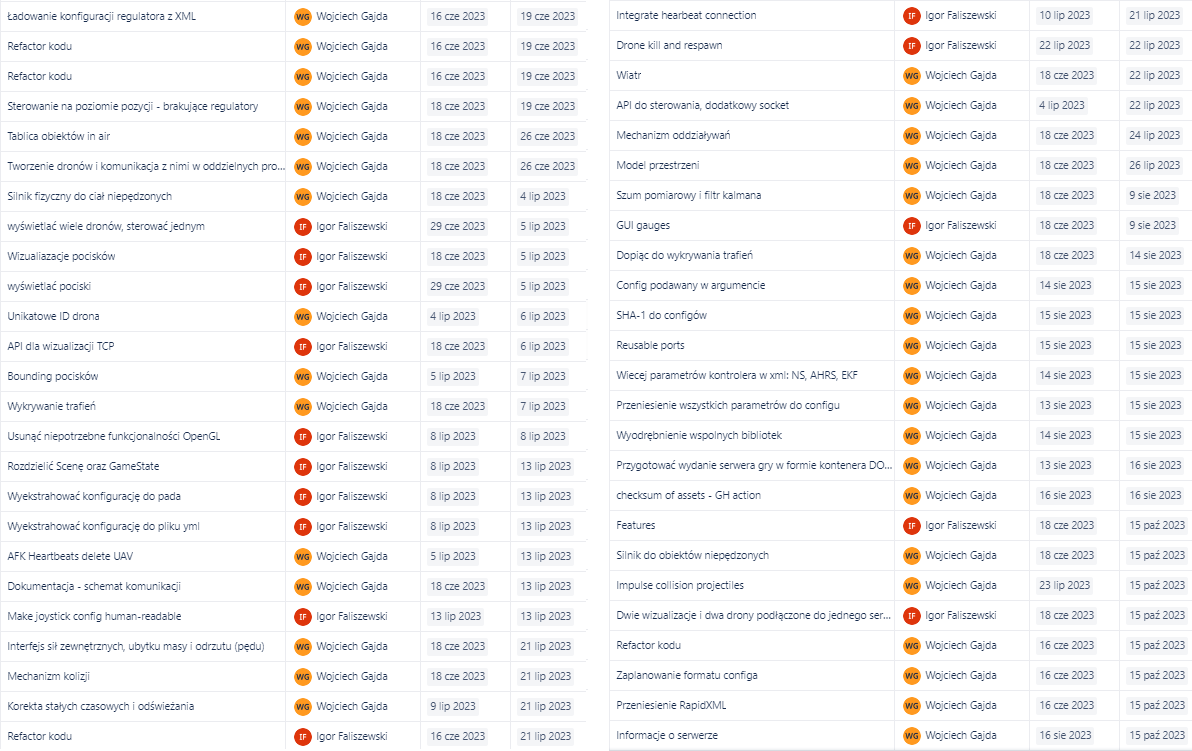
\includegraphics[width=\textwidth]{jira_june_sept.png}
\caption{Zgłoszenia zamknięte do 15.10.2023}
\label{zamkniete_jira}
\end{figure}

Na podstawie otwartych zagadnień i analizy założonej specyfikacji zaplanowany został harmonogram pracy zawierający zagadnienia, których realizacja jest niezbędna do ukończenia projektu. Tabela (\ref{harmonogram}) prezentuje ww. harmonogram. 

\renewcommand{\arraystretch}{1.5}
\begin{table}
\centering
\begin{tabular}{|m{0.4\textwidth}|m{0.15\textwidth}|m{0.15\textwidth}|m{0.2\textwidth}|} 
\hline
\rowcolor{Gray}
Opis zadania & Data\newline rozpoczęcia & Data\newline zakończenia & Osoba\newline odpowiedzialna \\
 \hline
Dodanie różnych modeli pocisków i ładunków & 16.10.2023 & 23.10.2023 & Igor Faliszewski \\
 \hline
Dodanie nowych konfiguracji rakiet & 16.10.2023 & 29.10.2023 & Wojciech Gajda \\
 \hline
Generator konfiguracji kontrolera & 24.10.2023 & 29.10.2023 & Igor Faliszewski \\ 
\hline
Implementacja nowych regulatorów płatowców & 30.10.2023 & 19.11.2023 & Wojciech Gajda \\ 
\hline
Krzywa łańcuchowa & 30.10.2023 & 12.11.2023 & Igor Faliszewski \\ 
\hline
Określanie orientacji pocisków i~ładunków & 13.11.2023 & 19.11.2023 & Igor Faliszewski \\ 
\hline
GUI wyboru pocisku i ładunku & 20.11.2023 & 26.11.2023 & Igor Faliszewski \\ 
\hline
Rozwój klasy regulatorów PID & 20.11.2023 & 10.12.2023 & Wojciech Gajda \\ 
\hline
Radio & 27.11.2023 & 03.12.2023 & Igor Faliszewski \\ 
\hline
Generowanie assetów na podst. map terenu & 04.12.2023 & 31.12.2023 & Igor Faliszewski \\ 
\hline
Nazwy użytkowników nad statkami & 04.12.2023 & 10.12.2023 & Igor Faliszewski \\
 \hline
Dodatkowe algorytmy całkowania & 11.12.2023 & 31.12.2023 & Wojciech Gajda \\
 \hline
Dźwięk gry & 11.12.2023 & 18.12.2023 & Igor Faliszewski \\
 \hline
Limit FPS & 19.12.2023 & 23.12.2023 & Igor Faliszewski \\
 \hline
Zachowanie kamery w pobliżu ściany & 26.12.2023 & 31.12.2023 & Igor Faliszewski \\ 
\hline
Dokumentacja kodu & 16.10.2023 & 31.12.2023 & Wszyscy \\ 
\hline
Testy & 13.11.2023 & 31.12.2023 & Wszyscy \\
 \hline
Rozbudowa assetów & 30.10.2023 & 31.12.2023 & Wszyscy \\ 
\hline
\end{tabular}
\caption{Harmonogram projektu październik -- grudzień 2023}
\label{harmonogram}
\end{table}

\newpage
\subsection{Ocena ryzyka -- analiza SWOT}

\begin{table}[!h]
\begin{tikzpicture}
\renewcommand{\arraystretch}{1.2}
\setlist{left=1em,parsep=0.5ex,after=\smallskip}
\def\myw{7.5cm}
\matrix[SWOT] 
{
\& |[fill=black!10]|\renewcommand{\arraystretch}{1.3}\begin{tabular}{Wc{\myw}Wc{\myw}}
Pozytywne & Negatywne\\ 
\end{tabular}\\
 Wewnętrzne
  \& \begin{tabular}{p{\myw}p{\myw}}
	\textbf{Silne strony:} \begin{itemize}
 	 \item przejrzysta implementacja zgodna z paradygmatami programowania obiektowego,
        	 \item modułowość projektu, pozwalająca na modyfikację poszczególnych komponentów bez konieczności przebudowy całego projektu,
        	 \item uniwersalny model dynamiki statków powietrznych, pozwalający na obliczenia w czasie rzeczywistym.
\end{itemize}
& 
 \textbf{Słabe strony:} \begin{itemize}
  	\item ograniczony czas projektu może skutkować niedopracowaniami we wdrożonych funkcjonalnościach,
        \item obliczenia symulacji i kolizji obywają się na CPU, co może ograniczać wydajność,
        \item model matematyczny jest mniej dokładny niż rozbudowana symulacja mechaniki płynów.
\end{itemize} \end{tabular}\\
 Zewnętrzne \& \begin{tabular}{p{\myw}p{\myw}}
	\textbf{Szanse:} \begin{itemize}
   	\item dzięki udostępnieniu systemu na otwartej licencji, możliwe jest wykorzystanie wypracowanych rozwiązań w przyszłych projektach,
       	\item system może stanowić narzędzie ułatwiające opracowanie i testowanie nowatorskich systemów sterowania,
       	\item system może stanowić bezpłatną alternatywę dla komercyjnych symulatorów lotu.
\end{itemize} & \textbf{Zagrożenia:} \begin{itemize}
  \item język Rust wykorzystany w UAV\_aggregator może przestać być wspierany na przestrzeni najbliższych lat,
  \item trudności z identyfikacja wiarygodnych współczynników modelu dynamiki,
  \item rozbudowany system może okazać się trudny w obsłudze dla użytkownika.
  
\end{itemize} \end{tabular}\\
};
\end{tikzpicture}
\caption{Analiza SWOT}
\label{swot}
\end{table}


\section{Testy oprogramowania}

Testowanie oprogramowania ma na celu weryfikację opracowanych rozwiązań. Odpowiednio przygotowane testy pozwalają na szybką detekcje błędu, a także rozwiązanie jego przyczyny. W zależności od przyjętej ideologi, testy oprogramowania przygotowywane są przed lub po opracowaniu właściwego kodu programu. Szczególnym przypadkiem testów pisanych po zakończeniu implementacji są testy pisane nigdy.\\

Metodyka realizacji testów jest dobrze rozwinięta dla typowych aplikacji webowych, co skutkuje dużym wyborem narzędzi umożliwiających testowanie i "mockowanie" modułów. W przypadku symulacji i gier komputerowych sytuacja jest odmienna. Oprócz sprawdzenia poprawności kodu niezbędna jest walidacja samego symulowanego modelu. Służą do tego specjalne mechanizmy, które wykształciły się w branży lotniczej.\\

Przygotowane testy można podzielić na cztery kategorie: testy jednostkowe, testy integracyjne, testy end-to-end oraz testy walidujące poprawność symulacji.

\subsection{Testy jednostkowe}

Testy jednostkowe to rodzaj testów oprogramowania, które sprawdzają indywidualne jednostki kodu, takie jak funkcje, metody czy klasy. Ich celem jest sprawdzenie, czy poszczególne fragmenty programu działają poprawnie, zgodnie z oczekiwaniami.
W programach zawierających elementy fizyki szczególnie ważne jest przetestowanie czy komponenty odpowiedzialne za przedstawienie poszczególnych zjawisk mają sens fizyczny.
W opracowanej symulacji kompleksowo przetestowane zostały obliczenia fizyczne, konwertery, klasa ODE, klasa Controller oraz model atmosfery ISA. 

\subsubsection{Testy klasy implementującej model atmosfery ISA}

Model wzorcowy atmosfery ISA (International Standard Atmosphere) to model matematyczny pozwalający na oszacowanie warunków atmosferycznych takich jak temperatura, ciśnienie oraz gęstość powietrza w zależności od wysokości nad poziomem morza. W bazowej formie pozwala na poprawne oszacowanie parametrów w warstwie przypowierzchniowej tj. troposferze. Testy klasy sprawdzają czy wartości obliczane przez klasę są zgodne z wartościami dostępnymi w tablicach. Analiza kilkunastu punktów testowych pozwala z dużym prawdopodobieństwem potwierdzić poprawność implementacji.

\subsubsection{Testy metod całkowania równań różniczkowych}

W klasie ODE znajduje się implementacja algorytmów całkowania równań różniczkowych. Główną funkcją w klasie jest funkcja \texttt{step(...)} wykonująca jeden krok całkowania. Testy dotyczące tej klasy pokrywają kwestie programowe takie jak poprawne tworzenie i dekonstrukcja klasy, ale także mają za zadanie sprawdzenie fizycznej poprawności tej klasy. W tym celu sprawdzone zostały następujące scenariusze:

\begin{enumerate}
\item funkcja prawych stron przyjmuje wartość stałą równą zeru. Sprawdzenie czy całkowana zmienna nie ulega zmianie
\item funkcja prawych stron przyjmuje wartość stałą. Jako, że każda z metod całkowania powinna być co najmniej pierwszego rzędy, sprawdzane jest czy rozwiązanie jest zgodne z analitycznym.
\item sprawdzenie liczby wywołań funkcji prawych stron. Każda z metod deklaruje liczbę niezbędnych wywołań funkcji prawych stron. Jako, że wywołania mogą być potencjalnie kosztowne, sprawdzane jest czy liczba wywołań jest zgodna z deklarowaną, optymalną liczbą wywołań wynikającą z teorii.
\item całkowanie równań różniczkowych opisujących oscylator harmoniczny bez tłumienia (masa na sprężynie). W trakcie całkowania w każdym kroku obliczana jest całkowita energia mechaniczna, będąca sumą energii kinetycznej i energii potencjalnej sprężystości. Sprawdzane jest czy całkowita energia mieści się w żądanym polu tolerancji, symetrycznym względem energii początkowej układu.
\end{enumerate}
 
\subsubsection{Testy implementacji regulatorów}

Interfejs Controller definiuje klasy reprezentujące różne regulatory wykorzystywane przez układ sterowania. Główną funkcją w interfejsie jest funkcja \texttt{calc(...)} obliczająca wyjście z regulatora dla przekazanej wartości zadanej i mierzonej zmiennej regulowanej. Do testów przygotowane zostały obiekty regulatorów z doświadczalnie dobranymi nastawami. Testy tej klasy mają na celu potwierdzić poprawność regulacji poprzez realizację następujących scenariuszy:

\begin{enumerate}
\item sprawdzenie czy znak wyjścia z regulatora jest zgodny ze znakiem uchybu tj. różnicy pomiędzy wartością zadaną, a wartością aktualną.
\item symulacja regulacji w układzie o jednym stopniu swobody, w którym wartość wyjściowa z regulatora wpływa na pochodną z zmiennej regulowanej. Scenariusz reprezentuje uproszczony model regulacji temperatury w pomieszczeniu z którego ucieka ciepło, a regulator steruje grzejnikiem dostarczającym ciepło. Badane jest czy po odpowiednim czasie ustalenia temperatura w pomieszczeniu utrzymuje się w założonym polu tolerancji. Dodatkowo w trakcie testu logowane są przebiegi wartości regulowanej. Ma to na celu umożliwić organoleptyczną analizę poprawności działania regulatora. Przykładowe przebiegi ilustruje rysunek (\ref{controller_plot}).
\end{enumerate}

\begin{figure}[!th]
	\centering
	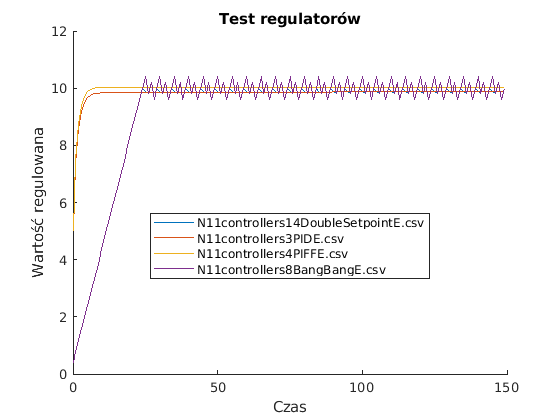
\includegraphics[width=0.7\textwidth]{controller_plot.png}
	\caption{Przebieg testu regulatorów}
	\label{controller_plot}
\end{figure}
\newpage

\subsection{Testy integracyjny}

Testy integracyjne są kolejnym etapem testowania oprogramowania, który koncentruje się na weryfikacji poprawności całościowego działania modułów systemu. Ich celem jest sprawdzenie, czy poszczególne części oprogramowania będą działać w połączeniu ze sobą. Polegają one najczęściej na uruchomieniu wybranego modułu w izolacji i sztucznym wygenerowaniu zapytań i odpowiedzi pochodzących z innych modułów. Rozbudowane testy integracyjne zostały napisane dla modułów UAV\_drop\_physic oraz UAV\_visualization. Fizyka obiektów jest testowana pod względem tworzenia nowych obiektów oraz ich reakcji na fizyczne bodźce. Testowanie wizualizacji przeprowadzone jest za pomocą skryptu w języku Python, który imitując serwer inicjalizuje wizualizację oraz wysyła dane, które tester jest w stanie zweryfikować na podstawie wygenerowanego obrazu.

\subsubsection{Testy modułu UAV\_drop\_physic}

Moduł \textbf{UAV\_drop\_physic} odpowiada za symulację lotu pocisków i ładunków, a wiec obiektów nie posiadających własnego źródła napędu. Testy modułu zawierają sprawdzenie poprawności uruchomienia i zamknięcia modułu, nawiązanie z nim komunikację, ale także sprawdzają poprawność działania przez symulację następujących scenariuszy testowych:

\begin{enumerate}
\item sprawdzenie mechanizmu dodawania i usuwania obiektów z symulacji. Sprawdzana jest poprawność nadawania identyfikatorów kolejnym obiektom,
\item symulacja spadku swobodnego bez oporu powietrza. Sprawdzane jest czy zmianie ulega jedynie składowa pionowa prędkości i położenia oraz czy wynik symulacji jest zgodny z rozwiązaniem analitycznym z przyjętą tolerancją.
\item symulacja spadku swobodnego z silnym oporem powietrza (spadochroniarz). Podobnie jak w powyższym teście sprawdzane jest osiągniecie określonej prędkości i położenia po zakładanym czasie.
\item symulacja wpływu siły zewnętrznej. Do spadającego swobodnie obiektu przyłożona zostaje pozioma siła. Sprawdzane jest czy horyzontalne składowe położenia odpowiadają rozwiązaniu analitycznemu dla ruchu przyspieszonego.
\item symulacja odbić od płaszczyzn, wykorzystywana w mechanizmie kolizji. Sprawdzane są odbicie plastyczne, sprężyste i sprężyste z tarciem. W każdym z testów sprawdzane są cechy charakterystyczne położenia i prędkości po odbiciu.
\item symulacja długotrwałego lotu w silnym wietrze. Dla obiektu na który działa silny wiatr poziomy oczekiwane jest, że po dostatecznie długim czasie osiągnie on prędkość zgodną z działającym wiatrem. 
\end{enumerate}
\subsubsection{Testy integracyjne wizualizacji}

Test integracyjny wizualizacji uruchomić można za pomocą skryptu \\ \texttt{visualization\_tests.py}, gdzie argumentami jest ścieżka do pliku wykonywalnego Javy, za pomocą której powinien zostać uruchomiony klient, katalog, w którym znajduje się klient, nazwa archiwum JAR klienta oraz suma kontrolna assetów, które wizualizacja ma wykorzystać. \\


Test rozpoczyna się od utworzenia wszystkich wymaganych gniazd sieciowych (socket'ów) obsługiwanych przez serwer. Następnie do katalogu klienta przekopiowywane są dane testowe w postaci konfiguracji aplikacji, przypisań kontrolera oraz parametrów drona i uruchamiana jest aplikacja. Skrypt następnie nawiązuje połączenie z aplikacją i testuje proces rozpoczęcia symulacji od pobrania przez klienta danych o serwerze, wysłaniu przez klienta odpowiednich parametrów BSP po jego prośbę o utworzenie statku. Po poprawnej wymianie informacji z aplikacją zmiany wprowadzone przez dane testowe są wycofane. Następnie skrypt przechodzi do wysyłania co 5ms wygenerowanego stanu BSP, który jest widoczny z poziomu ekranu wizualizacji. Rutyna obejmuje poruszanie się oraz obrotu statku we wszystkich osiach oraz fluktuację prędkości obrotowej każdego z silników.  

\subsection{Testy End-to-end}

Testy end-to-end (E2E) są rodzajem testów oprogramowania, które sprawdzają poprawność działania systemu jako całości, od rozpoczęcia działania aż do oczekiwanych wyników. W ramach testów end-to-end przetestowane zostało działanie serwera, który rozpoczyna swoje wywołanie od modułu UAV\_aggregator. Uruchamia on moduły symulacji fizyki i kontrolera, sprawdzając czy zainicjalizowały się poprawnie. 
Następnie generowana jest komunikacja z wizualizacją, symulująca wejście od użytkownika. Pozwala ona na przetestowanie reakcji systemu na przychodzące wiadomości.
Ostatecznie serwer wyłącza moduły i weryfikuje poprawne zatrzymanie wszystkich procesów. 

\subsection{Testy walidujące}

Testy walidacyjne moją na celu potwierdzić użyteczność symulacji. To na podstawie ich wyniku podjęta zostaje decyzja, czy wyniki symulacji są wiarygodne i mogą zostać wykorzystane w analizach. W praktyce przygotowywania symulatorów lotniczych walidacja stanowi ostatni etap metody 4M, której poszczególnymi etapami są:
\begin{itemize}[noitemsep]
\item Manoeuvre -- zaplanowanie i wykonanie eksperymentu
\item Measurement -- pomiar i rejestracja stanu statku powietrznego
\item Method -- dobór odpowiedniej metody identyfikacji i estymacja
\item Model -- symulacja przygotowanego modelu matematycznego
\item Walidacja modelu -- sprawdzenie poprawności przygotowanego modelu
\end{itemize}

Jedną z najpopularniejszych metod walidacji są analiza sensu fizycznego modelu oraz tzw. dowód zgodności. Analiza sensu fizycznego modelu polega na sprawdzeniu czy zachowanie symulowanego modelu w określonych scenariuszach odpowiada przewidywanym odpowiedziom. Do podstawowych badań należy sprawdzenie poprawności zachowania w reakcji na wychylenia powierzchni sterowych i położenia przepustnicy. Dodatkowa analiza kąta natarcia i ślizgu pozwala na porównanie wartości symulowanych z testami tunelowymi. Powyższe testy mają charakter lokalny, badający pewien podzbiór stanów BSP. W przeciwieństwie do tego na podjęcie całkowitego werdyktu pozwala dowód zgodności. Polega on na pełnym zarejestrowaniu stanu obiektu w locie i symulacji oraz sprawdzenie czy są one ze sobą zgodne z określoną tolerancją. Tolerancja ta może wynikać ze skończonej dokładności czujników pomiarowych, szumu przetwarzania lub tolerancji Maximum Unnoticeable Added Dynamics, czyli największego dopuszczalnego błędu, który pozostanie niezauważony przez doświadczonego użytkownika. Ostatni z parametrów jest szczególnie użyteczny w przypadku symulatorów do szkolenia pilotów.\\

Ze względu na charakter pracy, budowa symulacji w oparciu o badanie konkretnego modelu nie jest możliwa. Przyjęty model stanowi fuzję cech modeli pojawiających się w literaturze, dla których nie wszystkie współczynniki są jasno określone. Zatem z pominięciem powyższych etapów przygotowana symulacja nie odwzorowuje wiernie konkretnego statku. Nie zmienia to faktu, że uniwersalny model również może być weryfikowany, ze względu na zachowania, które powinny wystąpić zawsze, niezależnie od konfiguracji. W ten sposób można zaplanować zbiór testów manualnych które pozwalają szybko potwierdzić poprawność modelu. Przykładowe zachowania, które podlegają sprawdzeniu to:
\begin{itemize}[noitemsep]
\item BSP poprawnie odpowiada na wychylenia osi joysticka, przynajmniej co do kierunku obrotu.
\item BSP posiada cechy bryły sztywnej poruszającej się w powietrzu.
\item W przypadku statków stabilnych aerodynamicznie, BSP pozostaje stabilny w trakcie lotu: BSP sam minimalizuje ślizg, gasi prędkości kątowe lub je ogranicza.
\item W przypadku wielowirnikowców poprawnie realizowany jest zawis
\item W przypadku płatowców, do utrzymania wysokości przy prędkości przelotowej potrzebny jest dodatni kąt natarcia. W locie odwróconym wymagany kąt natarcia jest większy.
\end{itemize}

\section{Wdrożenie oprogramowania}
\subsection{Dokumentacja wydania}
\subsubsection{Wymagania systemowe}
Aplikacja serwera została przygotowana do natywnej pracy na maszynie z systemem UNIX. Mając na uwadze uniwersalność użytych języków (C++ oraz Rust) pojęte zostały próby przeniesienia serwera na system Windows, jednak wiązało się to z problemami z dostępnością bibliotek C++. Ostatecznie oficjalnie wspieranymi systemami, które pozwalają na natywne uruchomienie serwera są Ubuntu w wersji 22.04 i pochodne. \\

W celu zapewnienia szerszej zgodności serwera przygotowany został obraz Docker, bazujący na obrazie \texttt{ubuntu:latest}. Tak przygotowany obraz może zostać uruchomiony na dowolnej maszynie wspierającej konteneryzacje Docker. Ceną, którą należy zapłacić za rozszerzoną zgodność jest obniżona wydajność symulacji, ze względu na wirtualizację. Doświadczenie pokazuje, że spadek wydajności jest niewielki, zwłaszcza w najnowszych wersjach Dockera.\\

 Uruchomienie klienta wymaga posiadania systemu operacyjnego z powłoką graficzna opartą na oknach oraz obsługującego monitory i wirtualną maszynę Java. Docelowa maszyna musi również obsługiwać bibliotekę OpenGL.


\subsubsection{Wymagania sprzętowe}

Aplikacja serwera realizuje równoległe obliczenia dla każdego z klientów. Oprócz podstawowych wątków serwera, na każdego klienta aplikacji przypada dwa procesy symulujące fizykę i sterowanie. Z tego powodu zaleca się, aby maszyna na której zostanie uruchomiony serwer posiadała dwukrotnie więcej rdzeni logicznych niż maksymalna liczba podłączonych klientów. Dodatkowo należy zalecane jest zapewnienie co najmniej 8GB pamięci RAM. \\

Do poprawnej pracy klienta wymagane jest, aby procesor graficzny docelowej maszyny był zgodny z interfejsem OpenGL. Najstarszą testowaną wersją był OpenGL w wersji 4.5. Ze względu na wielowątkowość klienta zalecany jest co najmniej 4 rdzeniowy procesor, a ze względu na potencjalnie znaczne rozmiary mapy, co najmniej 8GB pamięci RAM i 2GB pamięci procesora graficznego.

\subsubsection{Wymagane biblioteki} \label{libraries}

Aplikacja serwera wykorzystuje zewnętrzne biblioteki C/C++ oraz Rust. Moduły napisane w języku C++ korzystają z bibliotek standardowych oraz następujących bibliotek zewnętrznych: Eigen 3, cxxopts, rapidXML, ZeroMQ i cppZMQ oraz gtest.
Moduły napisane w Rust wykorzystują m.in. biblioteki nalgebra, zmq, xmltree, merkletree, sha1 oraz serde\_yaml. Pełna lista wymaganych bibliotek Rust znajduje się w module agregatora w pliku \texttt{Cargo.toml}.
Aplikacja kliencka wykorzystuje m.in. biblioteki LWJGL, JOML oraz JeroMQ. Pełna lista wymaganych bibliotek Java znajduje się w module wizualizacji w pliku \texttt{build.gradle}.  Zastosowanie poszczególnych bibliotek zostało opisane w rozdziale (\ref{technologies}).



\subsection{Instrukcja instalacji}
\subsubsection{Instalacja serwera z wykorzystaniem Docker} \label{docker_server}

Serwer symulacji może zostać uruchomiony na dowolnej maszynie wspierającej kontenery Docker. Obraz zawierający najnowszą wersje serwera wraz ze wszystkimi wchodzącymi w jego skład modułami został zamieszony na platformie Docker Hub. Platforma gwarantuje utrzymanie obrazu przez co najmniej 6 miesięcy. Ze względu na ulotność tego repozytorium właściwy obraz zostanie również przekazany wraz z dokumentacją.\\

Maszyna na której zostanie uruchomiony serwer musi mieć zainstalowane i dostępne z poziomu wiersza poleceń następujące programy: \texttt{docker} oraz \texttt{docker compose}. Sprawdzenia, czy dana maszyna wspiera kontenery Docker można dokonać poprzez wydanie poleceń: \texttt{docker --version} i \texttt{docker compose version}. Niniejsza instrukcja została sprawdzona dla maszyny z zainstalowanym Docker w wersji 24.0.6 oraz Docker Compose w wersji v2.21.0. Szczegóły dotyczące instalacji Dockera można znaleźć na stronie projektu \cite{docker}\\

Instalację serwera należy rozpocząć od pobrania lub skopiowania na maszynę repozytorium \textbf{UAV\_server}. Repozytorium zostało udostępnione m.in. w serwisie GitHub. Jeśli maszyna na której ma być zainstalowany serwer ma zainstalowany program \texttt{git} to repozytorium może zostać pobrane przy poniższego polecenia:
\begin{lstlisting}[language=bash]
  $  git clone https://github.com/MiNI-UAV/UAV_server.git
\end{lstlisting}

W folderze repozytorium zamieszone zostały skrypty ułatwiające uruchomienie serwera. Przed uruchomieniem serwera należy jednak utworzyć odpowiednią strukturę plików i zasobów które będą wykorzystywane przez serwer. Służy do tego skrypt prepareVolume odpowiednio w wersji  \texttt{prepareVolume.sh} dla maszyn systemem z rodziny UNIX i  \texttt{prepareVolume.bat} dla maszyn z systemem Windows. Po uruchomieniu właściwego skryptu w folderze repozytorium utworzony zostanie folder \texttt{data}. Folder zawiera domyślne zasoby, przez zmianę których użytkownik może wpłynąć na działanie serwera mogące zostać.  Więcej informacji dotyczących zawartości tego folderu zostanie przedstawione w instrukcji obsługi (\ref{manual}).\\

Po zakończeniu konfiguracji serwer można uruchomić poniższym poleceniem wywołanym z folderu repozytorium:
\begin{lstlisting}[language=bash]
  $  docker compose up
\end{lstlisting}
Po uruchomieniu w wierszu poleceń pojawią się informację dotyczące pracy symulacji. Pierwszą linijką uruchomionej symulacji jest: \texttt{0.000 [Server] UAV SERVER}. Po zakończeniu uruchamiania serwer jest gotowy na obsługę klientów.\\

Prace serwera można zakończyć poprzez wysłanie do niego sygnału SIGINT. Można to zrobić skrótem klawiszowym \keys{\ctrl + C}. Jeśli serwer został uruchomiony w tle do zatrzymania należy wykorzystać właściwe polecenia Docker.

\subsubsection{Instalacja klienta z wykorzystaniem archiwum JAR}
\label{javaInst}

Klient może zostać uruchomiony na każdej platformie obsługującej maszynę wirtualną Java. 
Maszyna, na której zostanie zbudowany klient musi mieć zainstalowane Java Runtime Environment (JRE). Polecenie \texttt{java --version} pozwoli to sprawdzić. Informacja o wersji JRE znajduje się w drugiej linijce wyjścia. Instrukcja instalacji najnowszej wersji znajduje się na oficjalnej stronie projektu \cite{java}. Niniejsza instrukcja została sprawdzona dla JRE w wersji 17. \\

Instalację klienta należy rozpocząć od pobrania lub skopiowania na maszynę archiwum z aplikacją. Jest ono dostępne za pośrednictwem witryny GitHub na stronie \url{https://github.com/MiNI-UAV/UAV\_visualization/releases}. Archiwum powinno nazywać się \texttt{mini-uav-x.y.z}. Po jego rozpakowaniu należy wybrać katalog odpowiadający systemowi operacyjnemu i rozpakować do katalogu docelowego tam zawarte archiwum. \\

Przed uruchomieniem aplikacji warto zapoznać się z instrukcją obsługi zawartą w rozdziale \ref{fastClient}. \\

W przypadku systemu Windows włączenie aplikacji polega na uruchomieniu pliku wykonywalnego \texttt{MiniUAV.exe}. Na systemie Linux uruchomić aplikację można za pomocą następującego polecenia :

\begin{lstlisting}[language=bash]
  $ java -jar MiniUAV.jar
\end{lstlisting}

\subsubsection{Samodzielna budowa kodu serwera i natywna instalacja w systemie Ubuntu}

Serwer może zostać skompilowany natywnie i uruchomiony na maszynie z systemem UNIX. Na czas pisania tej instrukcji działanie serwera zostało przetestowanie z pozytywnym rezultatem na maszynach z zainstalowanym Ubuntu 22.04 oraz Pop! OS 22.04. Oba z testowanych systemów wykorzystują APT i w tej instrukcji opisany zostanie sposób pobrania bibliotek przy pomocy tego właśnie systemu zarządzania pakietami. W celu pobrania bibliotek opisanych w rozdziale (\ref{libraries}) należy wykonać poniższe polecenie instalujące niezbędne narzędzia:
\begin{lstlisting}[language=bash]
  $  sudo apt-get update && sudo apt-get install -y gcc g++ make cmake \ 
	build-essential curl autoconf automake libtool pkg-config libsodium-dev \
 	wget gitlibx11-dev software-properties-common && sudo apt-get update 
\end{lstlisting}

Następnie przy pomocy poniższych komend należy zainstalować właściwe biblioteki C++:
\begin{lstlisting}[language=bash]
  $  sudo apt-get install -y libcxxopts-dev libeigen3-dev libzmq3-dev \
	librapidxml-dev libgtest-dev 
  $  wget https://github.com/zeromq/cppzmq/archive/refs/tags/v4.10.0.tar.gz && \
    	tar -xvf v4.10.0.tar.gz && cd cppzmq-4.10.0 && mkdir build && cd build && \
    	cmake -DCMAKE_BUILD_TYPE=Release .. && make install && cd ../..
\end{lstlisting}

Następnie na maszynie należy zainstalować runtime języka Rust. Aktualny opis instalacji można znaleźć na stronie projektu Rust (\cite{rust_getting_started}). Poprawność instalacji języka Rust można sprawdzić przy pomocy polecenia \texttt{cargo --version}. Niniejsza instrukcja została przetestowana cargo w wersji 1.69.0.\\
 
Po zakończeniu instalacji bibliotek należy przejść budowy samego serwera. W trakcie pracy serwer korzysta z wielu modułów, które wzajemnie odnoszą się do swoich zasób. Kluczowym jest zatem, aby odpowiednie moduły znajdowały się w odpowiednim miejscu w hierarchii folderów. Zalecane jest zatem utworzenie pustego folderu (np. o nazwie UAV) w której znajdzie się serwer. W dalszej części instrukcji folder ten będzie nazywany folderem serwera. Do folderu serwera należy skopiować moduły \textbf{UAV\_physic\_engine}, \textbf{UAV\_controller}, \textbf{UAV\_drop\_physic} oraz \textbf{UAV\_aggregator}. Moduły można również sklonować z repozytorium GitHub przy pomocy poniższych poleceń wywołanych z folderu serwera:
\begin{lstlisting}[language=bash]
  $  git clone https://github.com/MiNI-UAV/UAV_aggregator.git 
  $  git clone https://github.com/MiNI-UAV/UAV_physics_engine.git
  $  git clone https://github.com/MiNI-UAV/UAV_controller.git
  $  git clone https://github.com/MiNI-UAV/UAV_drop_physic.git
\end{lstlisting}

Moduły \textbf{UAV\_physic\_engine}, \textbf{UAV\_controller} oraz \textbf{UAV\_drop\_physic} zostały napisane w języku C++ i do ich zbudowania należy wykorzystać program Cmake. W tym celu należy wejść kolejno do każdego z trzech powyższych folderów i wykonać następujące polecenia:
\begin{lstlisting}[language=bash]
  $  mkdir build
  $  cd build
  $  cmake ..
  $  make
  $  cd ../..
\end{lstlisting}
Spowoduje to utworzenie w każdym z modułów folderu build zawierającego plik wykonywany z programem. Należy sprawdzić czy w folderach build znajdują się pliki wykonywalne odpowiednio o nazwach: \texttt{uav}, \texttt{controller} oraz \texttt{drop}.

Na koniec należy zbudować modułu \textbf{UAV\_aggregator}. Po wejściu do folderu z modułem należy wykonać poniższe polecenie:
\begin{lstlisting}[language=bash]
  $  cargo build
\end{lstlisting}
Spowoduje to automatyczne pobranie niezbędnych bibliotek Rust i budowę kodu źródłowego.\\

W tym momencie wszystkie moduły potrzebne do pracy serwera zostały właściwie zbudowane. W celu uruchomienia serwera należy w folderze modułu\\ \textbf{UAV\_aggregator} wykonać następujące polecenie:
\begin{lstlisting}[language=bash]
  $  cargo run
\end{lstlisting}

Analogicznie jak w rozdziale (\ref{docker_server}) serwer został uruchomiony i czeka na klientów. W celu zamknięcia serwera należy wysłać sygnał SIGINT (\keys{\ctrl + C}). Wszystkie moduły zostaną zamknięte automatycznie.

\subsubsection{Samodzielna budowa kodu klienta i instalacja z wykorzystaniem Gradle}
 
Maszyna, na której zostanie zbudowany klient musi mieć zainstalowane Java Development Kit (JDK). Polecenie \texttt{java --version} pozwoli to sprawdzić. Informacja o wersji JDK znajduje się w pierwszej linijce wyjścia. Instrukcja instalacji najnowszej wersji znajduje się na oficjalnej stronie Oracle \cite{javaDown}. Ponadto maszyna powinna mieć zainstalowany program \texttt{Gradle}. To czy jest on zainstalowany sprawdzić można za pomocą polecenia \texttt{gradle --version}. Jego instalacja jest omówiona na stronie projektu \cite{gradle}. Niniejsza instrukcja została sprawdzona dla JDK w wersji 17 i Gradle w wersji 8.1.1 \\


Instalację klienta należy rozpocząć od pobrania lub skopiowania na maszynę repozytorium \textbf{UAV\_visualization}. Repozytorium zostało udostępnione m.in. w serwisie GitHub. Jeżeli maszyna ma zainstalowany program \texttt{git} to repozytorium może zostać pobrane za pomocą poniższego polecenia:

\begin{lstlisting}[language=bash]
  $  git clone https://github.com/MiNI-UAV/UAV_visualization.git 
\end{lstlisting}

W celu zbudowania projektu należy w katalogu repozytorium wykonać polecenie:

\begin{lstlisting}[language=bash]
  $  gradle build
\end{lstlisting} 

Po uruchomieniu serwera i skonfigurowaniu aplikacji jak opisano w rozdziale \ref{fastClient} aplikację można uruchomić za pomocą następującego polecenia:

\begin{lstlisting}[language=bash]
  $  gradle run 
\end{lstlisting}  

\newpage

\subsection{Instrukcja obsługi} \label{manual}

\subsubsection{Konfiguracja serwera przed uruchomieniem}

Przed uruchomieniem serwera możliwa jest zmiana ogólnych parametrów symulacji przez modyfikację pliku \texttt{config.yaml}. Plik ten znajduje się w folderze \texttt{configs} w module \textbf{UAV\_aggregator}. Dla wygody użytkowników serwera w wersji Docker, folder ten został połączony jako folder współdzielony z folderem \texttt{configs} znajdującym się w folderze \texttt{data} w folderze serwera.

Po otwarciu pliku \texttt{config.yaml} dowolnym edytorem tekstowym użytkownik ma możliwość zmiany parametrów serwera. Do najważniejszych parametrów należą:
 \begin{itemize}
\item parametr \texttt{map} pozwala na wybór mapy, na której prowadzona będzie symulacja. Mapa o podanej nazwie musi być dostępna w zasobach serwera. Więcej o zarządzaniu mapami zostanie wyjaśnione w rozdziale (\ref{add_map})
\item parametr \texttt{grid} pozwala na określenie ilości elementów w siatce w osi X, Y oraz Z. Odpowiedni dobór siatki poprawia jakość działania systemu wykrywania kolizji z mapą. Zalecane jest dobranie takiej ilości elementów, aby poszczególne \textit{chunki} były zbliżone do sześcianów o dł. krawędzi równej 30,
\item parametry \texttt{temperature}, \texttt{pressure}, \texttt{wind\_matrix} oraz \texttt{wind\_bias} pozwalają na skonfigurowanie początkowych warunków atmosferycznych i pola prędkości wiatru. 
\item parametry \texttt{*\_step\_time} pozwalają na ustawienie kroku obliczeń w poszczególnych modułach symulacji. Krok wyrażony jest w milisekundach.
\item parametry \texttt{*\_ode\_solver} pozwalają na wybór algorytmu całkowania równań różniczkowych wykorzystywanego w poszczególnych modułach.
\item parametry \texttt{*\_port} pozwalają na zmianę portów wykorzystywanych w komunikacji TCP. UWAGA: do poprawnej pracy zmiana portów wymagana jest również po stronie wizualizacji. Ponadto zmiana portów w serwerze w wersji Docker wymaga również przekierowania nowych portów w pliku \texttt{docker-compose.yml}.
\end{itemize}

Ponadto w pliku znajdują się inne, mniej istotne parametry. Kompletny opis parametrów znajduje się komentarzach pliku \texttt{config.yaml}.



\subsubsection{Uruchomienie serwera - Docker}

W celu uruchomienia serwera należy w folderze repozytorium \texttt{UAV\_server} wydać polecenie:
\begin{lstlisting}[language=bash]
  $  docker compose up
\end{lstlisting}
Po uruchomieniu w wierszu poleceń pojawią się informację dotyczące pracy symulacji. Pierwszą linijką uruchomionej symulacji jest: \texttt{0.000 [Server] UAV SERVER}. Po zakończeniu uruchamiania serwer jest gotowy na obsługę klientów.\\

Prace serwera można zakończyć poprzez wysłanie do niego sygnału SIGINT. Można to zrobić skrótem klawiszowym \keys{\ctrl + C}. Jeśli serwer został uruchomiony w tle do zatrzymania należy wykorzystać własciwe polecenia Docker.

\subsubsection{Uruchomienie serwera - Ubuntu}

Natywnie zbudowany serwer uruchamia się wydając w folderze modułu\\ \textbf{UAV\_aggregator} następujące polecenie:
\begin{lstlisting}[language=bash]
  $  cargo run
\end{lstlisting}

Analogicznie jak w poprzednim rozdziale serwer został uruchomiony i czeka na klientów. W celu zamknięcia serwera należy wysłać sygnał SIGINT (\keys{\ctrl + C}). Wszystkie moduły zostaną zamknięte automatycznie.

\subsubsection{Konfiguracja klienta przed uruchomieniem}
\label{fastClient}

Aby skonfigurować aplikację przed pierwszym uruchomieniem należy zmodyfikować plik \texttt{config.yaml} w module \textbf{UAV\_visualization}. Zaczynając od góry, w celu skonfigurowania kontrolera należy upewnić się, że zmienna \texttt{bindingsConfig.generateOnStartUp} jest ustawiona na \texttt{true} oraz w \texttt{bindingsConfig.source} znajduje się ścieżka względna do pliku, który zostanie utworzony w czasie konfiguracji i będzie zawierał ustawienia kontrolera. Zmienną \texttt{serverSettings.serverAddress} należy ustawić na adres IP serwera, na którym został postawiony serwer. Jeżeli chcemy pobrać assety z repozytorium GitHub, to zmienna \texttt{serverSettings.assetsSourceUrl} powinna być ustawiona na \texttt{https://github.com/MiNI-UAV/UAV\_aggregator/releases/download/}, zmienna \\ \texttt{serverSettings.downloadMissingAssets} na \texttt{true}, a zmienna \texttt{serverSettings.assetsToUse} powinna być zakomentowana. Jeżeli chcemy wykorzystać assety niezależne od tych, które proponuje serwer, to zmienna \texttt{serverSettings.downloadMissingAssets} powinna być ustawiona na  \texttt{false}, a zmienna \texttt{serverSettings.assetsToUse} na nazwę katalogu w folderze \texttt{assets} zawierającego zawartość, z której chcemy skorzystać. Następnie, \texttt{droneSettings.droneConfig} powinno wskazywać na plik w katalogu \texttt{drones}, który zawiera parametry BSP. Zmienna \texttt{droneSettings.modes} jest tablicą mówiąca o tym, jakie tryby kontroli lotu będą dostępne do wysłania serwerowi. Wraz z aplikacją dostępne są domyślne pliki parametrów wraz z utworzonymi dla nich trybami kontroli lotu, które widnieją w tabeli (\ref{modesTable}). Wszystkie dostępne tryby kontroli lotu są zdefiniowane przez serwer w katalogu assetów w podfolderze \texttt{data/available\_control\_modes.yaml}. Tak zmodyfikowana konfiguracja powinna być wystarczająca do rozpoczęcia pracy. W konfiguracji znajdują się inne mniej istotne parametry, których opis znajduje się w komentarzach.

\begin{table}[!ht]	
	\begin{center}
		\begin{tabular}{ |c|c| } 
			\hline
			Plik parametrów BSP & Dedykowane tryby kontroli lotu \\
			\hline
			\multirow{3}{7em}{quadcopter.xml} 
			& QPOS \\ & QANGLE \\ & QACRO \\
			\hline
			\multirow{3}{5em}{{plane.xml}} 
			& FANGLE \\ & FACRO \\ & FMANUAL \\
			\hline
			\multirow{1}{5em}{{rocket.xml}} 
			& RMANUAL \\
			\hline
		\end{tabular}
		\caption{Dedykowane tryby kontroli lotu dla domyślnych konfiguracji BSP}
		\label{modesTable}
	\end{center}
\end{table}

\subsubsection{Konfiguracja kontrolera przed uruchomieniem}

Jeżeli w konfiguracji pole \texttt{bindingsConfig.generateOnStartUp} zostało ustawione na \texttt{true}, to przy uruchomieniu aplikacji zostanie włączony generator konfiguracji. Ma on za zadanie przeprowadzić użytkownika przez proces utworzenia konfiguracji kontrolera. W pierwszej linijce widnieje nazwa pliku, który zostanie utworzony. Jeżeli żaden kontroler nie zostanie wykryty, użytkownik zostanie poproszony o jego podłączenie. Następnie użytkownik zostanie poproszony o ustawienie wszystkich osi oraz przycisków w położeniu domyślnym oraz naciśnięcie klawisza Enter (\keys{\return}). Obecne wartości osi i przycisków zostaną uznane za punkt zero (trim). Następnie generator konfiguracji wejdzie w tryb ustawiania osi sterowania. W drugiej linijce jest wyświetlona obecnie przypisywana oś. Pierwsze cztery osie domyślnie odpowiadają kolejno: ciągowi (throttle), pochyleniu (roll), przechyleniu (pitch) i odchyleniu (yaw). W nadzwyczajnych przypadkach możliwe jest przypisanie większej liczby osi. Przypisanie osi sterowania polega na wybraniu odpowiedniej osi poprzez jej wychylenie do wartości minimalnej i maksymalnej. Wybrana oś widoczna jest w linijce trzeciej, a wychylenia minimalne i maksymalne wraz z punktem zero w linijce czwartej. Po naciśnięciu klawisza Enter użytkownik zostanie poproszony o ustawienie za pomocą strzałek (\keys{\ \arrowkeyleft}, \keys{\arrowkeyright}) deadzone osi oraz następnie czy oś ma być odwrócona. Ostatecznie należy nacisnąć klawisz Enter aby przejść do następnej osi. Po skalibrowaniu przynajmniej czterech domyślnych osi należy nacisnąć klawisz Esc (\keys{\esc}). Wtedy użytkownik zostanie poproszony o przypisanie akcji. Do każdej akcji może zostać przypisana dowolna liczba osi, przycisków i klawiszy. Nazwa obecnie przypisywanej akcji oraz numer przypisania jest wyświetlony w linijce drugiej. Przypisanie klawisza polega na wciśnięciu odpowiedniego klawisza na klawiaturze i naciśnięciu Enter. Wybrany klawisz zostanie wyświetlony w linijce trzeciej. Przypisanie przycisku wygląda analogicznie. Przypisanie osi polega najpierw na wykryciu wybranej osi, naciśnięciu Enter oraz ustawieniu za pomocą strzałek wartości minimalnej i maksymalnej osi przy, której nastąpi aktywacja akcji. Obecna wartość osi jest wyświetlona w linijce trzeciej. Zakończenie przypisania osi następuje po ustawieniu obydwu wartości i naciśnięciu Enter. Po przypisaniu wybranej liczby przypisań do danej akcji, użytkownik może przejść do akcji następnej poprzez naciśnięcie klawisza Esc. Warto zauważyć, że nie jest wymagane ustalenie przypisań dla wszystkich akcji. Ostatnim krokiem konfiguracji kontrolera jest ustawienie przypisań trybów kontroli lotu. Ich numeracja odpowiada kolejności, w której zostały zdefiniowane w konfiguracji klienta w polu \texttt{droneSettings.modes}. Ich przypisanie przechodzi w sposób podobny do akcji, z taką różnicę, że przy pierwszym przypisaniu do trybu klawisz Esc kończy konfigurację trybów, a przy każdym kolejnym przypisaniu do trybu klawisz Esc pozwala przejść do przypisania trybu kolejnego. Wynika z tego to, że tryb powinien mieć co najmniej jedno przypisanie, by móc przypisać tryby następne.

\subsubsection{Uruchomienie klienta}

W przypadku systemu Windows włączenie aplikacji polega na uruchomieniu pliku wykonywalnego \texttt{MiniUAV.exe}. Na systemie Linux uruchomić aplikację można za pomocą następującego polecenia :

\begin{lstlisting}[language=bash]
	$ java -jar MiniUAV.jar
\end{lstlisting}

\subsubsection{Odczytanie logów z symulacji}

W trakcie symulacji serwer rejestruje ("loguje") stan poszczególnych BSP oraz ogólny stan symulacji. Wszystkie zarejestrowane informacje znajdują się w folderze \texttt{logs} w module \textbf{UAV\_aggregator}. Dla wygody użytkowników serwera w wersji Docker, folder ten został połączony jako folder współdzielony z folderem \texttt{logs} znajdującym się w folderze \texttt{data} w folderze serwera. W folderze logi z poszczególnych symulacji zostały podzielone na foldery, których nazwy odpowiadają nazwą sesji. Nazwą sesji jest liczba będąca datą uruchomienia serwera w postaci Unix Timestamp. W folderze odpowiadającym konkretnej sesji znajdują się: folder \texttt{drop\_physic} zawierający plik \texttt{state.csv}, plik \texttt{server.log} oraz foldery odpowiadające lotom wykonanym w ramach sesji. Plik \texttt{state.csv} zawiera kolejne pozycje i prędkości obiektów symulowanych przez moduł \textbf{UAV\_drop\_physic}. Plik \texttt{server.log} zawiera zapis z konsoli serwera. Pojawią się w nim informacje o rozpoczęciu i zakończaniu lotu, a także komunikaty przekazane wprost z silnika fizyki i modułu sterowania.\\

Foldery z lotami noszą nazwy związane z nazwą drona i zawierają dokładnie jeden lot. Jeśli klient resetował stan BSP, kolejny lot zawarty zostanie w nowym folderze. W każdym z folderów znajdują się pliki CSV z zarejestrowanymi parametrami lotu oraz odpowiadające wygenerowanym charakterystykom. Poniżej przedstawiona została lista ww. plików wraz z opisem:

 \begin{itemize}[noitemsep]
\item \texttt{accelerometer.csv} -- pomiary symulowanego czujnika przyśpieszenia tj. przyśpieszeniomierza,
\item \texttt{ahrs.csv} -- orientacja BSP estymowana przez system AHRS,
\item \texttt{aoa.csv} -- charakterystyka pochodnych aerodynamicznych w funkcji kąta natarcia,
\item \texttt{aos.csv} -- charakterystyka pochodnych aerodynamicznych w funkcji kąta ślizgu,
\item \texttt{atmosphere.csv} -- warunki atmosferyczne zarejestrowane przez BSP,
\item \texttt{barometer.csv} -- pomiary symulowanego czujnika ciśnienia atmosferycznego tj. barometru,
\item \texttt{EKF.csv} -- pozycja BSP estymowana przez system nawigacji oparty o rozszerzony filtr Kalmana,
\item \texttt{env.csv} -- rzeczywisty stan BSP (pozycja, prędkość, orientacja itd.) będący wynikiem symulacji,
\item \texttt{GPS.csv} -- pozycja BSP wyznaczona przez symulowany system nawigacji satelitarnej,
\item \texttt{GPSVel.csv} -- prędkość BSP wyznaczona przez symulowany system nawigacji satelitarnej,
\item \texttt{gyroscope.csv} -- pomiary symulowanego czujnika prędkości kątowej tj. żyroskopu,
\item \texttt{magnetometer.csv} -- pomiary symulowanego natężenia pola magnetycznego tj. magnetometru,
\item \texttt{rotors.csv} -- zarejestrowane wartości prędkości kątowe silników rotorowych.
\end{itemize}



\subsubsection{Dodanie nowego BSP}

Wszystkie parametry dotyczące symulowanego BSP zostały zawarte w pliku XML, którego nazwa odpowiada nazwie konkretnego statku. Plik XML znajdują się po stronie klienta w module \textbf{UAV\_visualization} w folderze \texttt{drones}. Domyślnie do projektu zostały dołączone pliki z parametrami wielowirnikowca, stałopłatowca i rakiety, odpowiednio o nazwach \texttt{quadcopter.xml}, \texttt{plane.xml} oraz \texttt{rocket.xml}. Dodatkowo folder zawiera plik \texttt{aircraft\_template.xml} który nie reprezentuje żadnego konkretnego BSP, ale zwiera wszystkie z możliwych parametrów wraz w właściwymi opisami w komentarzach XML.\\

W celu utworzenia nowego BSP należy skopiować najbardziej zbliżony do oczekiwanego plik XML i zapisać go w folderze \texttt{drones} pod unikatową nazwą i rozszerzeniem XML. Następnie należy zmodyfikować wybrane parametry. Do najważniejszych parametrów należą:

 \begin{itemize}[noitemsep]
\item parametr \texttt{name} -- określający nazwę BSP w symulacji,
\item parametr \texttt{type} -- określający teksturę i siatkę 3D statku wykorzystywaną w wizualizacji i kolizjach,
\item parametry z grupy \texttt{initial} -- określają startową pozycję, prędkość i orientację BSP, a także tryb sterowania w chwili uruchomienia,
\item parametry z grupy \texttt{ineria} -- określają własności masowe BSP,
\item parametry z grupy \texttt{rotors} -- określają silniki wirnikowe,
\item parametry z grupy \texttt{jets} -- określają silniki marszowe,
\item parametry z grupy \texttt{surface} -- określają powierzchnie sterowe,
\item parametry z grupy \texttt{aero} -- określają własności aerodynamiczne BSP,
\item parametry z grupy \texttt{controllers} i \texttt{mixers} -- określają regulatory i miksery wykorzystywane przez system sterowania,
\item parametry z grupy \texttt{navi} -- określają parametry systemu nawigacji,
\item parametry z grupy \texttt{ammo} -- określają amunicję przenoszoną przez BSP,
\item parametry z grupy \texttt{cargo} -- określają ładunki przenoszone przez BSP,
\end{itemize}

Model 3D podany w parametrze \texttt{type} musi być dostępny w zasobach serwera. Jeśli żaden z domyślnych modeli nie odpowiada przygotowywanej konfiguracji, nowy typ może zostać dodany do zasobów serwera w następujący sposób:

\begin{enumerate}
	\item w katalogu \texttt{drones} utworzyć folder o nazwie zgodnej z zawartością parametru \texttt{type}.
	\item w nowo utworzonym katalogu dodać podfoldery \texttt{model} i \texttt{textures}.
	\item w folderze \texttt{model} umieścić model 3D w formacie GTLF (\texttt{model.gltf}) wraz z odpowiadającym mu plikiem binarnym (\texttt{model.bin}) oraz w formacie OBJ (\texttt{model.obj}). Układ współrzędnych powinien znajdować w środku masy BSP i być układem NED.
	\item W folderze \texttt{textures} powinny znajdować się wszystkie tekstury, do których odnosi się model. Należy upewnić się, że plik GLTF uwzględnia katalog \texttt{textures} w referencjach do tekstur.
\end{enumerate}

\subsubsection{Dodanie nowej mapy} \label{add_map}

 W celu dodania nowej mapy do zasobów należy:
 
 \begin{enumerate}
 	\item w katalogu \texttt{maps} utworzyć folder o nazwie, która będzie jednoznacznie identyfikować mapę.
 	\item w nowo utworzonym katalogu dodać podfoldery \texttt{model} i \texttt{textures}.
 	\item w folderze \texttt{model} umieścić model 3D mapy w formacie GTLF (\texttt{model.gltf}) wraz z odpowiadającym mu plikiem binarnym (\texttt{model.bin}) oraz w formacie OBJ (\texttt{model.obj}). Przyjętym układem współrzędnych jest układ NED.
 	\item w folderze \texttt{model} dodatkowo powinien się znaleźć plik \texttt{minimap.png}, który będzie wykorzystywany podczas wyświetlania minimapy. Ma to być kwadratowa tekstura, gdzie każdy piksel odpowiada jednemu metru kwadratowemu, a jej środek odpowiada koordynatom (0,0).
 	\item W folderze \texttt{textures} powinny znajdować się wszystkie tekstury, do których odnosi się model. Należy upewnić się, że plik GLTF uwzględnia katalog \texttt{textures} w referencjach do tekstur.
 \end{enumerate}

\subsubsection{Aktualizacja zasobów serwera}

Do zapewnienia poprawnej pracy klienta i serwera kluczowe jest aby obie strony dysponowały identycznymi zasobami. Zasoby znajdują się folderze \texttt{assets} w module \textbf{UAV\_aggregator} oraz w podfolderach folderu \texttt{assets} w module \textbf{UAV\_visualization} (wizualizacja może posiadać kilka zasobów, rozróżnialnych hashem). W trakcie uruchamiania serwer oblicza hash dla wykorzystanych zasobów i przekazuje go do podłączających się wizualizacji. Ponadto w przygotowany został pipeline CICD, który po przesłaniu nowej wersji assetów, wydaje paczki assetów na platformie GitHub. Jeśli klient nie posiada assetów o wskazanej nazwie, bedzie próbował pobrać je właśnie z GitHuba.\\

Jeśli program uruchamiany jest lokalnie należy ręcznie skopiować zasoby wykorzystywane przez serwer do klienta. W tym celu należy:
\begin{enumerate}
\item uruchomić serwer,
\item znaleźć w folderze \texttt{configs} plik o nazwie \texttt{assets\_checksum} i odczytać hash zasobów,
\item skopiować z serwera cały folder \texttt{assets} do folderu \texttt{assets} w module\\ \textbf{UAV\_visualization},
\item zmienić nazwę folderu na pierwsze 8 znaków odczytanego hasha zasobów,
\item uruchomić aplikację kliencką.
\end{enumerate}

\chapter{Podsumowanie pracy}


W ramach pracy pomyślnie opracowano kompleksowy system umożliwiający symulację lotu bezzałogowych statków powietrznych. Wszystkie założone cele zostały osiągnięte, a zachowanie symulowanych statków nie wykazuje niezgodności z rzeczywistością.\\

Realizacja pracy pozwoliła poszerzyć umiejętności z zakresu projektowania i implementacji systemów komputerowych, ale także umożliwiła zanurzenie się w różnych aspektach lotnictwa oraz grafiki komputerowej. Zgromadzona wiedza obejmuje nie tylko techniczne aspekty tworzenia oprogramowania, lecz także praktyczne aspekty funkcjonowania bezzałogowych statków powietrznych. Do realizacji projektu potrzebne było zdobycie wiedzy z zakresu fizyki, mechaniki lotu oraz teorii sterowania. Realizacja wielu aspektów symulacji wymagała zastosowania odpowiedniego podejścia, które pozwoliło na przeniesienie teoretycznej wiedzy do działającego oprogramowania. Zbadane zostało wiele technik renderowania trójwymiarowej grafiki komputerowej dostępnych w specyfikacji OpenGL. Zrealizowany projekt nie wyczerpuje jednak możliwości tego interfejsu. Powyższą pracę można traktować jako porządne wprowadzenie do ogólnych technik renderowania grafiki trójwymiarowej. Będzie ona stanowić fundament wiedzy potrzebnej w przyszłych projektach wykorzystujących narzędzia pokrewne takie jak WebGL lub bardziej zaawansowane jak Vulkan. \\

Praca ta może być wykorzystana jako podstawa dalej rozwijanego systemu, zmodyfikowanego pod potrzeby konkretnego odbiorcy. Przygotowana baza kodu może stanowić podwaliny kolejnych, wyspecjalizowanych systemów. Dzięki dużej dbałości o przejrzystość kodu i pełnej dokumentacji, rozwój tego oprogramowania powinien być znacznie ułatwiony, Istnieje wiele zagadnień, które mogą w przyszłości zostać uwzględnione w rozwijanym systemie, a samego tematu z pewnością nie można uznać za zamknięty.

\section{Załączniki}

\begin{itemize} %[noitemsep,nolistsep]
\item UAV\_physic\_engine\_doc.pdf -- dokumentacja modułu UAV physic engine
\item UAV\_drop\_physic\_doc.pdf -- dokumentacja modułu UAV drop physic
\item UAV\_controller\_doc.pdf -- dokumentacja modułu UAV controller
\item UAV\_common\_doc.pdf -- dokumentacja wspólnej biblioteki dla modułów napisanych w języku C++
\item UAV\_aggregator\_doc.zip -- dokumentacja modułu UAV aggregator w formie strony HTML.
\item UAV\_visualization\_doc.zip -- dokumentacja modułu UAV visualization w formie strony HTML.

\item aircraft\_template.xml -- szablon pliku konfiguracyjnego statek powietrzny
\item aggregator\_config.yaml -- szablon pliku konfiguracyjnego modułu aggregator
\item visualization\_config.yaml -- szablon pliku konfiguracyjnego modułu wizualizacji
\item bindings\_template.yaml -- szablon pliku konfiguracyjnego kontroler
\item available\_control\_modes.yaml -- szablon pliku konfiguracyjnego trybów lotu
\end{itemize}


\newpage
\section{Bibliografia}

%\printbibliography
\nocite{*}

\printbibliography[type=book,heading=subbibliography,title={Literatura}]
\printbibliography[type=article,heading=subbibliography,title={Artykuły}]
\printbibliography[type=online,heading=subbibliography,title={Źródła internetowe}]


\end{document}
